%\documentclass{article}
\documentclass{article}
\usepackage{times}
%\usepackage{natbib}
%\usepackage{multicol}
\RequirePackage{natbib}
\usepackage{amsmath, amssymb, fullpage, amsthm, array, algorithm2e,graphicx,asa}
%\usepackage[dvips]{graphics}

\graphicspath{{images/}}
\usepackage{color}
\newcommand{\blue}[1]{{\color{blue} #1}} %MM
\newcommand{\red}[1]{{\color{red} #1}} 
\newcommand{\green}[1]{{\color{green} #1}} %DC

\definecolor{orange}{rgb}{1,0.5,0}
\newcommand{\hh}[1]{{\color{orange} #1}} %HH

% \usepackage{pifont} % this package is used to print check mark \checkmark

\setlength{\oddsidemargin}{0in}
\setlength{\evensidemargin}{0in}
\setlength{\textwidth}{6.5in}
\setlength{\topmargin}{-0.4in}
\setlength{\textheight}{9in}
\evensidemargin 
\oddsidemargin

\newtheorem{thm}{Theorem}[section]
\newtheorem{dfn}{Definition}[section]
\newtheorem{cor}{Corollary}[thm]
\newtheorem{con}{Conjecture}[thm]
\newtheorem{lemma}[thm]{Lemma}

%\topmargin -0.10in   % when making pdf
%\textheight 9.15in  % when making pdf

\begin{document}

% Article top matter
\title{Validation of Visual Statistical Inference, Applied to Linear Models}
\author{Mahbubul Majumder, Heike Hofmann, Dianne Cook\\
        Department of Statistics, Iowa State University}
%\date{\today}  %\today is replaced with the current date
\maketitle

\begin {abstract}  
Statistical graphics play a crucial role in exploratory data analysis, model checking and diagnosis. Until recently there were no formal visual methods in place for determining statistical significance of findings. This changed, when \citet{buja:2009} conceptually introduced two protocols for formal tests of visual findings. In this paper we take this a step further by comparing the lineup protocol \citep{buja:2009} against classical statistical testing  of the significance of regression model parameters. A human subjects experiment is conducted using simulated data to provide controlled conditions. Results suggest that the lineup protocol provides results comparable to the conventional tests, out-performs them when data is contaminated, and, there may be some super-individuals who yield better power than the conventional test even in the most difficult trials.
\end {abstract}

%\begin{multicols}{2}
%\twocolumn

\section{Introduction} 

%\checkmark

Statistical graphics nourishes the discovery process in data analysis: revealing unexpected things,  finding structure that was not previously anticipated,  or orthogonally contrasting prevailing hypotheses. It is often associated with exploratory data analysis, which was pioneered by \cite{tukey:eda} and, is particularly pertinent in today's data-rich world where discovery during data mining has become an important activity. Graphics are also used in many places where numerical summaries simply do not suffice: model checking, diagnosis, and in the communication of findings. 

Statistical graphics research and development is agreeably established now, and has been cemented by several new developments in recent years. Early studies on evaluating how well statistical plots are perceived and read by the human eye \citep{cleveland:1984}, have been repeated and expanded \citep{heer:2010} with findings supporting the original results. This body of work provides a framework for evaluating new statistical graphics.  In a complementary direction, new research on formalizing statistical graphics with language characteristics makes it easier to abstractly define, compare and contrast data plots. \cite{wilkinson:1999} developed a grammar of graphics that is enhanced by \cite{hadley:2009}. These methods provide a mechanism to abstract the way data is mapped to graphical form. Finally, technology advances make it simple and easy for everyone to draw plots of data, and particularly the existence of software systems, such as R \citep{R}, enable making beautiful data graphics that can be tightly coupled with statistical modeling.

However, measuring the strength of patterns seen in plots, and differences in individual perceptual ability, is something that is difficult and perhaps handicaps graphics  use among statisticians, where measuring probabilities is of primary importance. This has also been addressed in recent research. \citet{buja:2009} proposes a protocol that allow the testing of discoveries made from statistical graphics. This work represents a major advance for graphics, because it bridges the gulf between classical statistical inference procedures and exploratory data analysis. One of the protocols, the lineup, places the actual data plot among  a page of plots of null data, and asks a human judge to pick the plot that is different. Figure \ref{fig:test_category} shows an example lineup. Which plot do you think is the most different from the others? (The position of the actual data plot is provided in Section \ref{sec:category}.) Wrapped in a process that mirrors classical inference, where there is an explicit, a priori, null hypothesis, picking the plot of the data from the null plots represents a rejection of that null hypothesis. The null hypothesis typically derives from the task at hand, or the type of plot being made. The alternative encompasses all possible antitheses, all types of patterns that might be detected in the actual data plot, accounting for all possible deviations from the null without the requirement to specify these ahead of time. The probability of rejection can be quantified, along with Type I, and Type II error, and $p$-value and power can be defined and estimated. 


\begin{figure}[htp]
%\begin{figurehere}
   \centering
       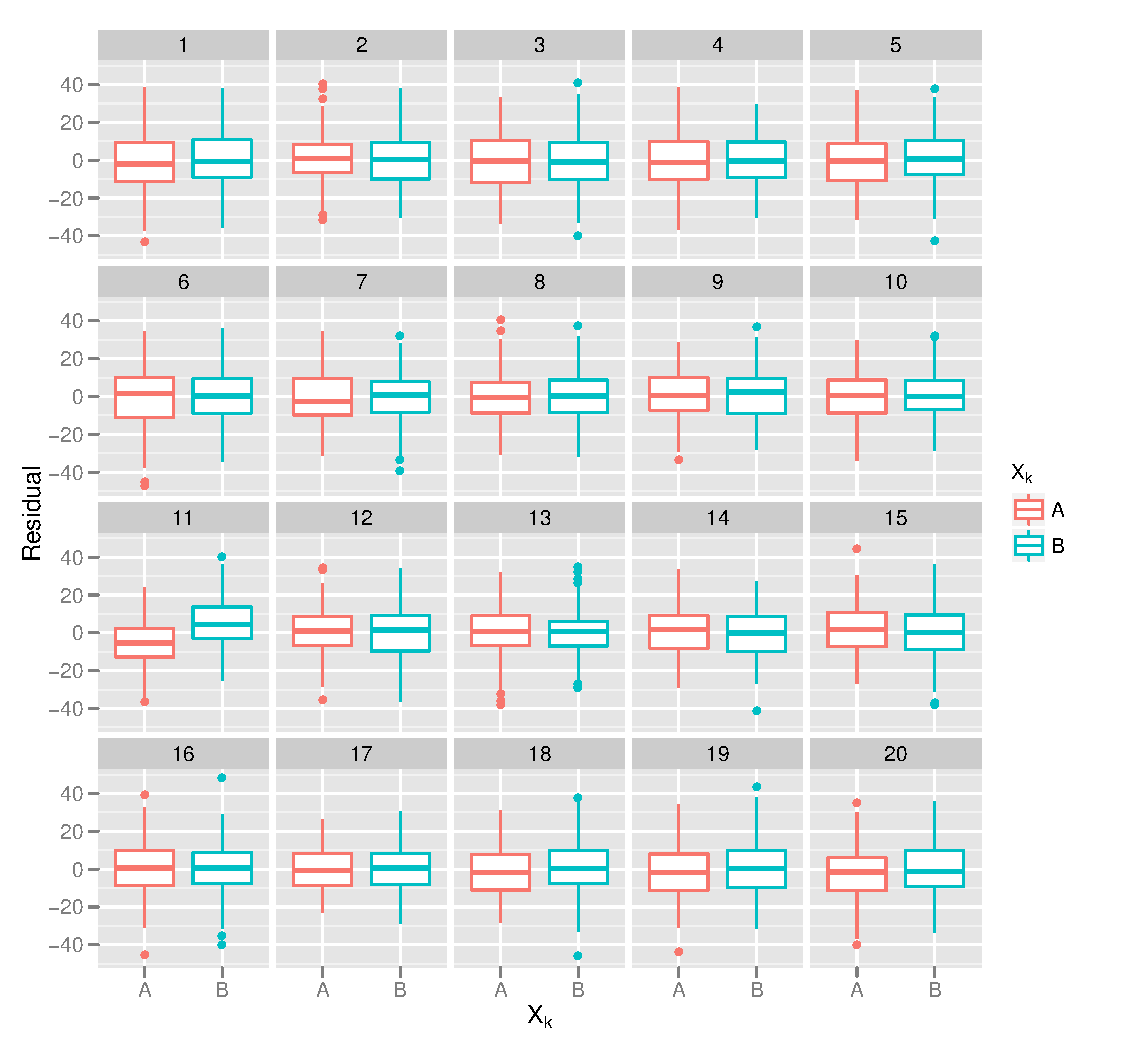
\includegraphics[width=0.95\textwidth]{lineup_category.pdf}
       \caption{Lineup plot ($m=20$) using side-by-side boxplots for testing $H_0: \beta_k=0$. One of these plots is the plot of the actual data, and the remaining are null plots, produced by simulating data from a null model that assumes $H_0$ is true. Which plot is the most different from the others, in the sense that there is the the largest shift or location difference between the boxplots? (The position of the actual data plot is provided in Section \ref{sec:category}.)}
       \label{fig:test_category}
\end{figure}
%\end{figurehere}

The protocol has only been informally tested until now. In the work described in this paper, the lineup protocol is compared head to head with the equivalent classical test. Specifically, the lineup is examined in the context of a linear model setting, where we are determining the importance of including a variable in the model. This is not the envisioned environment for the use of the lineup -- actually it is likely the worst case scenario for visual inference. The intended use of lineups is where there is no existing test, and unlikely to be ever any numerical test. The thought is though, that the classical setting provides a benchmark for how well the lineup protocol works under controlled conditions, and will provide some assurance that they will work in scenarios where there is no benchmark. Testing is done using a human-subjects experiment using Amazon's Mechanical Turk \citep{turk}, using simulation to provide controlled conditions for assessing lineups. The results are compared with those of the classical test. 

%, analysis requires plots of data. For exploratory data analysis, statistical graphics play an invaluable role in model checking and diagnostics. Even though we have established mathematical procedures to obtain various statistics, we need to support the results by also producing the relevant plots. 

%The scientific foundation of graphical methods for data analysis is well established by \cite{cleveland:1984}. In recent years we have seen several major advances in statistical graphics. Modern computing systems like R and SAS ease the production of high quality statistical plots. A grammar of graphics introduced by \cite{wilkinson:1999} presents a structured way to generate specific graphics from data and define connections between disparate types of plots.  \cite{hadley:2009} has implemented a revised version of the grammar of graphics in R, in the package {\tt ggplot2}.   \blue {Graham Wills has implemented the grammar in SPSS, but I'm not sure how to cite this.}


%\citet{buja:2009}, following from \cite{gelman:2004}, proposed two protocols that allow the testing of discoveries made from statistical graphics. This work represents a major advance for graphics, because it bridges the gulf between classical statistical inference procedures and exploratory data analysis.

%In this paper we compare the lineup protocol to classical statistical inference, specifically applied to the regression framework. We also present results of a human-subject study assessing the performance of individuals on lineup plots \citep{buja:2009} for testing significance of regression parameters. 

The paper is organized as follows. Section \ref{sec:visual_test} defines terms as used in visual inference, and describes how to estimate the important quantities from experimental data. The effect of the lineup size and number of observers on the power of the test is discussed in Section \ref{sec:size}. Section \ref{sec:regression} focuses on the application of  visual inference to linear models.  Section \ref{sec:simulation} describes the results of the three simulation experiments conducted to compare the power of the lineup protocol with the equivalent conventional test and an analysis of the resulting data. The last section describes the next steps in this research.


\section{Definitions and Explanations for Visual Statistical Inference} \label{sec:visual_test} 

Table \ref{tbl:compare} illustrates the lineup protocol in relation to traditional hypothesis testing. Both start from the same place, the same null hypothesis. The classical test statistic is the $t$-statistic, where the parameter estimate is divided by its standard error. In the lineup protocol, the test statistic is a plot of the data, here side-by-side boxplots are used, because the variable of interest is categorical and takes just two values. In traditional hypothesis testing the value of the test statistic is compared with all possible values of the sampling distribution, the distribution of the statistic if the null hypothesis is true. If it is extreme on this scale then the null hypothesis is rejected. In contrast in visual inference, the plot of the data is compared with plots of a finite number of samples drawn from the null distribution. If the actual data plot is selected as the most different, then this results in rejection of the null hypothesis.

\begin{table*}[hbtp]
\caption{Comparison of visual inference with existing inference technique.  }
\centering 
\begin{tabular}{llll} 
\hline
  & Traditional Inference &  Lineup Protocol \\ %[0.5ex] % inserts table %heading 
\hline
  Hypothesis & $H_0: \beta=0$ vs $H_1: \beta > 0$& $H_0: \beta=0$ vs $H_1: \beta > 0$\\
 & \begin{minipage}[h]{2.5cm} \begin{center} \scalebox{0.2}{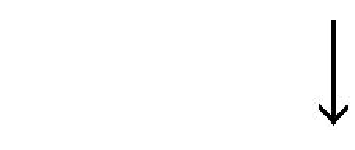
\includegraphics{down_arrow.pdf}} \end{center} \end{minipage} & \begin{minipage}[h]{2.5cm} \begin{center} \scalebox{0.2}{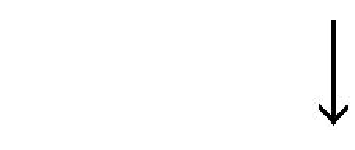
\includegraphics{down_arrow.pdf}} \end{center} \end{minipage} \\
				  
 Test statistic & $T(y)=\frac{\hat{\beta}}{se(\hat{\beta})}$ & $T(y)=$ \begin{minipage}[h]{1cm} \begin{center} \scalebox{0.45}{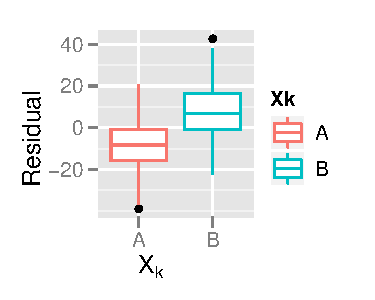
\includegraphics{stat_category.pdf}} \end{center} \end{minipage} \\
				 
 & \begin{minipage}[h]{2.5cm} \begin{center} \scalebox{0.2}{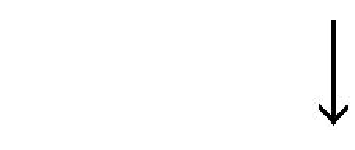
\includegraphics{down_arrow.pdf}} \end{center} \end{minipage} & \begin{minipage}[h]{2.5cm} \begin{center} \scalebox{0.2}{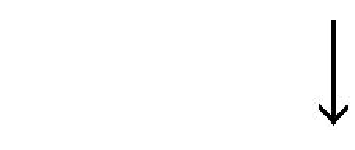
\includegraphics{down_arrow.pdf}} \end{center} \end{minipage} \\
				 
 Sampling Distribution & $f_{T(y)}(t); $\begin{minipage}[h]{2.5cm} \begin{center} \scalebox{0.55}{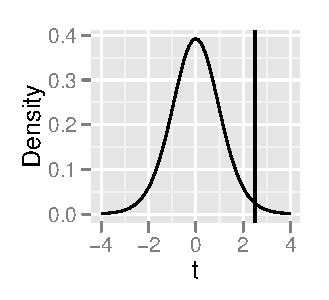
\includegraphics{stat_mathematical_test.pdf}} \end{center} \end{minipage} & $f_{T(y)}(t); $ \begin{minipage}[h]{2.5cm} \begin{center} \scalebox{0.32}{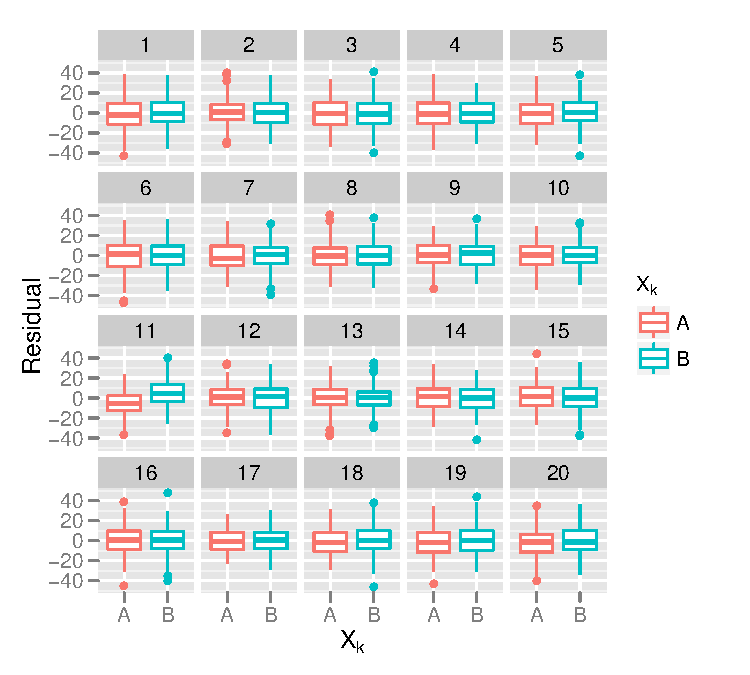
\includegraphics{lineup_category_small.pdf}} \end{center} \end{minipage} \\
 & \begin{minipage}[h]{2.5cm} \begin{center} \scalebox{0.2}{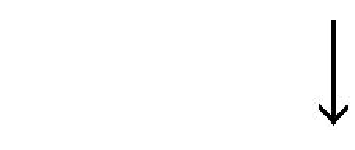
\includegraphics{down_arrow.pdf}} \end{center} \end{minipage} & \begin{minipage}[h]{2.5cm} \begin{center} \scalebox{0.2}{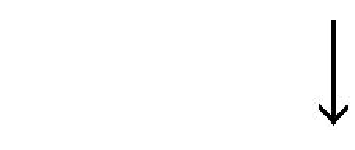
\includegraphics{down_arrow.pdf}} \end{center} \end{minipage} \\
 Reject $H_0$ if & actual $T$ is extreme & actual plot is identifiable \\
\hline 
\end{tabular}
\label{tbl:compare}
\end{table*}	


%Visual tests are non-parametric tests of the form $H_0$: the data plot is visually not distinguishable from a null plot vs $H_1$: the data plot is visually distinguishable from a plot generated consistently with $H_0$.

%Power of a plot and $p$-value have been derived in Buja and Wickham as ...



%for this paper, we want to place the parametric inference of a regression setting into the framework of visual testing:



%This section outlines the concepts of visual inference in comparison to the procedures of classical statistical inference. Table \ref{tbl:compare} (derived from \citet{buja:2009}) gives a summarized overview of this comparison.

In general, we define $\theta$ to be a population parameter of interest, with $\theta \in \Theta$, the parameter space. Any null hypothesis $H_0$ then partitions the parameter space into $\Theta_0$ and $\Theta_0^c$, with $H_0: \theta \in \Theta_0$ versus $H_1: \theta \in \Theta_0^c$. A test statistic, $T(y)$, is a function that maps the sample into a numerical summary, that can be used to test the null hypothesis. The hypothesis test maps the test statistic into \{0, 1\}, based on whether $T(y)$ falls into the acceptance region, or the rejection region, respectively. $T(y)$ is assessed relative to null values of this statistic $T(y_0)$ which would be possible values of $T$ if $\theta \in \Theta$.  %Similarly, for any test statistic, we have a rejection region $R$ and, complementary to that, $R^c$,  that partitions the space of the test statistic, which is usually a subspace of the real numbers. 
For visual inference, unlike in the classical hypothesis test, the statistic is not a single value, but a graphical representation of the data chosen to display the strength of the parameter of interest, $\theta$. When the alternative hypothesis is true, it is expected that the plot of the actual data, the test statistic, will have visible feature(s) consistent with $\theta \in \Theta_0^c$, and that visual artifacts will not distinguish the test statistic as different when $H_1$ is not true. We will call a plot with this property a {\it visual statistic} for $\theta$. More formally, 

\begin{dfn} \label{dfn:test}
A \textbf{visual test statistic}, $T(.)$, is a function of a sample that makes a plot. $T(y)$ maps the actual data to the plot, and we call this the \textbf{actual data plot}, and $T(y_0)$ maps samples drawn from the null distribution into the same plot form, and these are called \textbf{null plots}. 
\end{dfn}

\noindent Ideally, the visual test statistic is defined and constructed using the grammar of graphics \citep{wilkinson:1999,hadley:2009}, consisting of type, and specification of aesthetics, necessary for complete reproducibility. The visual test statistic is compared with values $T(y_0)$ using a lineup, which is defined as:

\begin{dfn}\label{dfn:lplot}
A \textbf{lineup} is a layout of $m$ randomly placed visual statistics, consisting of 
\begin{itemize}\itemsep-3pt
\item $m-1$ statistics, $T(y_0)$, simulated from the model specified by $H_0$  (null plots) and 
\item the test statistic, $T(y)$, produced by plotting the actual data, possibly arising from $H_1$.
\end{itemize}
\end{dfn}

\noindent The $(m-1)$ null plots can be members of the sampling distribution of the test statistic assuming that the null hypothesis is true. If $H_1$ is true, we expect this to be reflected as a feature in the test statistic, i.e. the plot of the data, that makes it visually distinguishable from the null plots. A careful visual inspection of the lineup by %\strikethrough{an} 
independent observers follows;  observers are asked to point out the plot most different from the lineup. If the test statistic is identified in the lineup, this is considered as evidence against the null hypothesis. 
%If it is not identified the conclusion is to not reject the null hypothesis. 

This leads us to a definition for the $p$-value of a lineup: under the null hypothesis, each observer has a $1/m$ chance of picking the test statistic from the lineup.  For $K$ independent observers, let $X$ be  the number of observers picking the test statistic from the lineup. Under the null hypothesis $X \sim \text{Binom}({K, 1/m})$,  therefore: 

\begin{dfn}\label{dfn:pvalue}
The $p$-value of a lineup of size $m$ is given as 
\[
P(X \ge x) = 1 - \text{Binom}({K, 1/m}) (x-1) = \sum_{i=x}^{K} {K \choose i} \left(\frac{1}{m}\right)^{i} \left(\frac{m-1}{m}\right)^{K-i},
\]
with $X$ defined as above. 
\end{dfn}
Note that for $x=0$ the $p$-value becomes --mathematically-- equal to 1. It might make more sense from a practical point of view to think of the $p$-value as
being larger than $P(X \ge 1)$ in this situation. If we increase either $m$ or $K$, we would be able to determine the value at a higher precision.

\noindent Table \ref{pvalue} shows $p$-values for different numbers of observers for lineups of size $m = 20$. It can be seen that, if the null hypothesis is true, it is unlikely that multiple observers would pick the actual data plot.

\begin{table}[htp]
\caption{Possible $p$-values for different numbers of observers, $K$, for fixed size $m = 20$ lineups.}
\begin{center}
\begin{tabular}{rrrrrrrrrrrrrrrrrrr}
$K$ &  $x$ & $p$-value && $K$ &  $x$ & $p$-value && $K$ &  $x$ & $p$-value && $K$  & $x$ & $p$-value && $K$  & $x$ & $p$-value\\ \cline{1-3} \cline{5-7}\cline{9-11}\cline{13-15}\cline{17-19}
1 &  1 & 0.0500 && 2 &  1 & 0.0975 && 3 & 1 & 0.1426 && 4 & 1 & 0.1855 && 5 & 1 & 0.2262 \\%\cline{1-3}
&&&& 2 &  2 & 0.0025 && 3 & 2 & 0.0073 && 4 & 2 & 0.0140 && 5 & 2 & 0.0226 \\
&&&& &&&& 3 & 3 & 0.0001 && 4 & 3 & 0.0005 && 5 & 3 & 0.0012 \\%\cline{1-6}
&&&&  &    &        &   &   &        &&& 4 & 4 & $< 0.0001$ && 5 & 4 & $< 0.0001$ 
\end{tabular}
\end{center}
\label{pvalue}
\end{table}

%\begin{dfn}\label{dfn:test}
%\red{why do we need the $\theta$? - it's not defined and not explained. usually we would assume that lineups are non-parametric}
%The \textbf{visual test}, $V_{\theta}$, is defined to be 
%\begin{itemize}\itemsep-3pt
%\item \textbf{Reject} $H_0$ if `enough' observers select the actual data plot in the lineup of $m$ plots, and
%\item \textbf{Fail to reject} $H_0$  otherwise. %if the observer selects a null plot.
%\end{itemize}
%where `enough' observers is defined as some threshold $x_{1-\alpha}$, for which $P(X \ge x_{1-\alpha}) < \alpha$, the level of significance.
%\end{dfn}

%\blue{To avoid confusion with one tailed $(1-\alpha)$ vs two tailed $(1-\alpha/2)$ notation, can we just use $x_{\alpha}$? }

%\red{alternative definition of visual test where $type-I$ error $\alpha$ is attached.}

\begin{dfn}\label{dfn:test}
The \textbf{visual test}, $V_{\theta}$  of size $\alpha$, is defined to be 
\begin{itemize}\itemsep-3pt
\item \textbf{Reject} $H_0$ if out of $K$ observers $x_{\alpha}$ of them correctly identify the actual data plot in the lineup, and
\item \textbf{Fail to reject} $H_0$  otherwise. %if the observer selects a null plot.
\end{itemize}
where $x_{\alpha}$ is such that $P(X \ge x_{\alpha}) < \alpha$. 
\end{dfn}

Associated with any test is the risk of making a Type I error, or Type II error, which for visual inference are defined as follows: 

\begin{dfn}\label{dfn:error}
The \textbf{Type I error} is the probability of rejecting $H_0$ when it is true, the probability for that is $P(X \ge x_{\alpha})$, which is controlled by $\alpha$.
% identifying the actual data plot, when $H_0$ is true, which is $1/m$, and is thus controlled by the number of null plots. 
\textbf{Type II error} is the probability of failing to identify the actual data plot, when $H_0$ is not true, $P( X <  x_{\alpha})$.
\end{dfn}

\green{Oh, we are using observed and observer, which might be confusing. May need to change observed data plot to something else. Will think about this. Will use ``actual'' for now.}

\noindent Because $X$ takes only discrete values we can not always control exactly for $\alpha$, with an exact $x_{\alpha}$. For example, when there is only one observer, $1/m$ is the minimal value at which we can set $\alpha$. It can be set to be smaller, even arbitrarily small, by increasing $K$. Type II error is harder to calculate, as is usually the case. In visual inference, individual abilities need to be incorporated to calculate Type II error. This is not necessary for Type I error, because it is simply the chance that the observer picks the actual data plot, by chance. For Type II error, we need to calculate the chance that the observer sees that actual data plot as different, when it really is different. This involves understanding the individual's visual skills. Thus, let $X_i$ be a binary random variable with $X_i = 1$, if individual $i (=1, \dots , K)$ identifies the actual data plot from the lineup, and $X_i = 0$ otherwise, where $p_i$ is the probability that individual $i$ picks out the actual data plot from the lineup. If all individuals have the same ability, with the probability, $p$, for picking out the actual data plot, then $X = \sum_i X_i$ has distribution $\text{Binom}(K, p)$. We can estimate $p$ by $\hat{p} = x/K$, where $x$ is the number of observers (out of $K$), who pick out the actual data plot from the lineup. 

\hh{If there is evidence for individual skills influencing the probability $p_i$, then $X_i \sim Binom_{1, p+i}$ and $X$ is a sum of independent Bernoulli random variables with different success rates $p_i$. This makes the distribution of $X$ a Poisson-Binomial by definition, see \citet{butler93} for details. estimating $p_i$ will be one of the main concerns for the remainder of the paper.}

%\green{WHY??? And how does this relate to the logistic model below?} 
%This leads to the definition of the power of the visual test, as follows:





%The lineup plot can be evaluated by one or more individuals. When a single individual identifies the observed graph in the lineup plot we report a $p$-value of at most $1/m$, otherwise the $p$-value is at least $1-\frac 1m$. 

 %Notice that when $N=1$, this $p$-value is $\frac1m$. 

%\subsection{Power}


%Next, we will develop power theoretically and then relate it to the empirical results.
%We will first theoretically define and  derive the power of  a visual test in the setting of a parametric hypothesis test, i.e. we assume a test  of $H_0: \theta = 0$ vs $H_1: \theta \neq 0$ for some real valued parameter vector $\theta$. In a next step we will then relate the theoretical results to our empirical findings.

%\red{How are $\Theta_0$ and $\Theta^c_0$ defined? - why do we need them? wouldn't it be better to re-formulate power in terms of acceptance region, not in terms of the parameter space? - $1/m$ also doesn't look right for the power - I think that's just looking at one observer.}
%\begin{dfn} \label{dfn:power}
%The \textbf{power} of a visual test $V_{\theta}$ is defined as the probability to reject the null hypothesis for a given parameter value $\theta$:
%    \begin{equation*}
%      \text{Power}_V(\theta)= 
%        \begin{cases} 
%              \frac1m & \text{if $\theta \in \Theta_0$,} \\
%              Pr(\text{Reject } H_0) &\text{if $\theta \in \Theta^c_0$.}
%        \end{cases}
%    \end{equation*}
%\end{dfn}
%
%
%\red{Alternative Power definition:}
\begin{dfn} \label{dfn:power}
The \textbf{power} of a visual test $V_{\theta}$ is defined as the probability to reject the null hypothesis for a given parameter value $\theta$:
    \begin{equation*}
      \text{Power}_V(\theta)= Pr(\text{Reject } H_0 \mid \theta) 
%      = P(X \ge x_{\alpha}) =
%        \begin{cases} 
%               1 - \text{Binom}_{K, 1/m}(x_{\alpha} - 1) & \text{ if } H_0 \text{ is true}.\\
%              1 - F_{X, \theta} (x_{\alpha} - 1) & \text{ if } H_1 \text{ is true}.
%        \end{cases}
    \end{equation*}
\end{dfn}

\hh{\noindent An important difference between classical testing and the lineup scenarios is that lineups always depend on observers -- this brings the number of people evaluating a particular lineup into the actual evaluation of power, i.e. we are assuming, again, that $X$ counts the number of observers (out of $K$) who identify the data plot from the lineup.
Then power is calculated as
\[
\widehat{Power}_{V} (\theta) = {Power}_{V, K} (\theta) = 1 - F_{X, \theta} (x_{\alpha} - 1),
\] 
where $F_{X, \theta}$ is the distribution of $X$ -- this depends on which hypothesis is true:

Under the null hypothesis $X \sim Binom_{K, 1/m}$, leading to a power of 
\[
\text{Power}_V(\theta, K)= 1 - Binom_{K, 11/m} (x_\alpha - 1),
\]
where $x_\alpha$ is defined as in (\ref{dfn:test}), as  $P(X \ge x_{\alpha}) < \alpha$.

If the alternative hypothesis is true with a fixed parameter value $\theta$, we can assume that an individual's probability to identify the data plot depends on the parameter value, and $X_i \sim Binom_{1, p_i(\theta)}$. Again, assessing an individual's probability to identify the data plot  is central to the actual calculation .
}
%\noindent Note that $F_{X, \theta}$ is the distribution of $X$ under the alternative with given parameter value $\theta$.

%\red{there may be a flow in this definition. Due to the discrete nature of binomial (specially $x_{\alpha}$) this definition would only give a conservative lower limit of the actual power. I feel like we should not define power using binomial.}

Power is an important consideration in deciding which test to use for solving a problem. %In classical testing, new test procedures are examined for their power under a variety of scenarios. 
For visual inference, this corresponds to the choice of plot to use. Analysts typically have a choice of plots to make, and a myriad of possible options such as reference grids, for any particular purpose. This is akin to different choices of statistics in classical hypothesis testing, for example, mean, median, or trimmed mean. One is typically better than another. For two different visual test statistics of the same actual data, one is considered to be better, if $T(y)$ is more easily distinguishable to the observer. Power is typically used to measure this characteristic of a test. %Power is the probability of rejecting $H_0$ when it is not true.  We can assess power therefore both empirically based on experimental data and through theoretical considerations. 

\section{Effect of Lineup Size and Number of Observers}~\label{sec:size}

\green{Notation changes $i$ to $j$, and $p$ to $\pi$. Can someone please decide which to use, and make the appropriate changes? How does the ``Let $X_{j\ell} \sim B_{1, \pi_{j\ell}}$...'' below relate to the ``let $X_i$ be a binary random variable...'' above? It looks like this is a repeat. One needs to go once notation is clarified.}

\red{Here is what my suggestion for notation \\  Use $B$ for logistic model and $\beta$ for linear model \\ Use $X$ to indicate logistic model covariate matrix and $U$ to denote binomial variable \\ $Y$ to indicate observed data. \\ Use $\pi_i$ instead of $p_i$ since $p_i$ is used for p-value.  \\ Should I change everything accordingly? I see that we have been careful not to use $\beta$ for power! }

\paragraph{Subject-specific abilities}
Calculating the power  is intricately related to the probability to identify the data plot from the lineup. 

Suppose each of $K$ independent observers gives evaluations on multiple lineups and responses are associated with binary random variable $X_{\ell i}$, where  $X_{\ell i} = 1$, if subject $i$ correctly identifies the test statistic on lineup $\ell$,  $\ell = 1, ..., L$, and 0 otherwise.

\hh{
We model $p_{\ell i} = E(X_{\ell i})$ as  a mixed effects logistic regression
 accommodating both for different abilities of individuals as well as differences in the difficulty of lineups: 


Let $X_{\ell i} \sim Binom_{1, p_{\ell i}}$ be the random variable, with $X_{ \ell i}= 1$, if  subject $i$ correctly identifies the data plot from lineup $\ell$, and 0 otherwise.
We can model $p_{ \ell i}$ with a logistic regression with subject specific random effects as:
\begin{equation} \label{mixed}
g( p_{\ell i} )= X_{\ell i} B +  Z_{\ell i}  \tau_{\ell i},  
\end{equation}

where $g(.)$ denotes the {\it logit} link function $g(\pi)=\log(\pi) - \log(1-\pi); 0 \le \pi \le 1$ and

\begin{tabular}{lp{5.5in}}
$X$  & is a design matrix of covariates corresponding to specifics of lineup $\ell$ and subject $i$. Covariates could include  demographic information of individuals, such as age, gender, education level etc. as well lineup-specific elements, e.g. difficulty level. \\
$B$ & is a vector of parameters for fixed effects.\\
$Z_{\ell i}$ & $1 \le i \le K$, $1 \le \ell \le L$  is a design matrix corresponding to random effects specific to individual $i$ and lineup $\ell$.  \\
$\tau$ & is a vector of independent real-valued random variables $\tau_{\ell i}$,  $\tau  \sim  MVN(0,\sigma_\tau I_{KL \times KL})$. $\tau$ will usually include a component incorporating an individual's ability or skill to evaluate lineups.\\
\end{tabular}

}



%\red{This model is  described in more detail in equation \ref{mixed}.}

%\noindent For any single observer, the power of a visual test has a lower limit of $\frac1m$ since the probability that an observer will randomly pick the test statistic under $H_0$ is $\frac1m$. When $K$ individuals evaluate a lineup plot independently, the number of successful evaluations, $U \sim \text{Binom} (K,1/m)$  under $H_0$. This leads us to obtain the probability 
%\begin{equation}\label{eqn:pvalue}
%Pr(U \ge u)= \sum_{k \ge u}^K {{K \choose k} \left(\frac{1}{m}\right)^k\left(1-\frac 1m\right)^{(K-k)}}
%\end{equation}
%where $u$ is the observed number of successful evaluations. We use this probability to  define the $p$-value for visual test $V_{\theta}$ as follows:
%\begin{dfn} \label{dfn:pval}
%The $p$-value associated with the decision of a visual test $V_{\theta}$ is given \blue{as the probability to observe a value at least as extreme as the test statistic $u$, 
%where $u$ is the number of successful evaluations of the lineup, which leads us to a $p$-value of $P(U \ge u)$ as given in eqn (\ref{eqn:pvalue}). Since $u$ is a discrete value with boundaries 0 and $K$,
% we can also re-formulate the $p$-value in terms of upper and lower boundaries:
% \begin{equation*}
% \begin{array}{rcll}
% P(U \ge u+1) \le &p\text{-value}& (\le 1), & \text{if }u < K, \text{and in particular for } u=0\\
%( 0 \le) &p\text{-value}& \le P(U \ge u-1), & \text{if }u > 1, \text{and in particular for } u=K.\\ 
% \end{array}
% \end{equation*}
% }
 
%\red{HH: Tried to re-write it to answer the question below.
%Why is the $p$ value not just $Pr(U \ge u)$ ? (We need to modify this a bit with respect to the rejection region $R$, but there should not be a difference in terms of whether we reject or accept. }
%
%    \begin{equation*}
%        \begin{cases} 
%              p\text{-value} \le Pr(U \ge u)    & \text{when reject $H_0$,} \\
%              p\text{-value} > 1-Pr(U \ge u)  & \text{when fail to reject $H_0$}
%        \end{cases}
%    \end{equation*}
%\end{dfn}


%\red{HH: the following paragraph needs some adjustment in terms of t and $\theta$ - could you try to take of that, Mahbub?}\\
%\red{For the following paragraph, we wanted to get rid of the absolute value of $t$ and instead look at $t \in R$ and $t \in R^c$.}

\noindent
\paragraph{Lineup size $m$}
One of the big differences between visual inference and the classical testing situation is the use of a finite number $m-1$ of representatives of the null distribution as comparison against the test statistic. The choice of $m$ has an obvious impact on the test, and we will discuss this in the following paragraph.

The following properties are only derived for the situation of a  fully parameterized  simulation study. This allows us to directly compare lineup tests against their classical counterparts and also identify  properties relevant for a quality assessment of  lineups, which are typically used  in non-parametric situations.

We need to make two crucial assumptions:
\begin{enumerate} \itemsep 0in
\item  the plot setup is structured in a way that makes it possible for observer to identify a deviation from the null hypothesis,
\item an observer is able to identify the plot with the strongest `signal' (or deviation from $H_0$)  from a lineup.
\end{enumerate}
We will be able to show evidence for the second assumption with the help of the study discussed in Section~\ref{sec:simulation}, \hh{the degree to which the first assumption is fulfilled is reflected} by the power of a lineup. The better suited a design is for a particular task, the higher its power will be.

\hh{In order to compare power of classical tests and lineups side-by-side, we will have to assume, that we are in the controlled environment of a simulation with tests corresponding to a known parameter value $\theta \in R$ and associated distribution function $F_t$ of the test statistic. }

\begin{lemma}~\label{lemma}
Suppose $F_{|t|}(.)$ is the distribution function of an absolute value of $t$, the classical test statistic. Suppose the associated test statistic in a classical test is observed as  $t_{obs}$ with $p$-value $p_D$. 

The probability of picking the data plot from a lineup depends on the size $m$ of the lineup and the strength of the signal in the data plot. 
Under the above assumptions, we can express the probability as:
\[
P(p_D < p_0) =  E\left[ (1 - p_D)^{m-1}\right]
\]
where $p_D$ is the $p$-value associated with the data in the test statistic, and $p_0$ is the minimum of all $p$-values in the data going into null plots.
\end{lemma}

\begin{proof}
We will now make use of properties of the data going into the lineup and assume that the properties are reflected in the lineup display:

 By definition we have 

$$p_D=Pr\left(|t| \ge t_{obs} \mid H_0\right)=1-F_{|t|}(t_{obs}) \ \ \Rightarrow \ \  |t_{obs}|=F_{|t|}^{-1}(1-p_D)$$

%Now suppose $F_{|t|}(.;\delta)$ denotes the distribution function of an absolute value of $t$, the classical test statistic.
%, with non-centrality parameter $\delta$. 
Then the distribution function of the $p$-value $p_D$ under $H_0$ is uniform, since:  
\begin{eqnarray}\label{dist_p}
F{p_D}(p) &=& Pr(p_D \le p)=1-Pr(1-p_D \le 1-p) \nonumber \\
  &=& 1-Pr\left(F_{|t|}^{-1}(1-p_D) \le F_{|t|}^{-1}(1-p) \right) \nonumber \\
  &=& 1-Pr\left(|t_{obs}| \le F_{|t|}^{-1}(1-p)\right) \nonumber \\
  &=&%\left\{ \begin{array}{ll}
          1-F_{|t|}\left( F_{|t|}^{-1}(1-p)\right)=p \mbox{ ; under $H_0$} 
 %         1-F_{|t|}( F_{|t|}^{-1}(1-p); \delta) &\mbox{ ; under $H_1$} 
%       \end{array} \right.     
\end{eqnarray}

%Thus the density of $p_D$ is Uniform(0,1)  under $H_0$. As noted by \cite{Ruppert:2007}, under $H_1$ the density of $p_D$ $$f_{p_D}(p_D; \delta)= \frac{f_{|t|}(F_{|t|}^{-1}(1-p_D);\delta)}{f_{|t|}(F_{|t|}^{-1}(1-p_D))}$$ derived from equation \ref{dist_p}  is a right skewed distribution.  



Let $p_{0,i}$, $i=1, ..., m-1$ denote the  $p$-values associated with data corresponding to the $m-1$ null plots. Since this data is generated consistently with the null hypothesis,  the $p$-values are independent and  follow a standard Uniform distribution, $p_{i,0} \sim U[0,1], i= 1, ..., m-1$.

\hh{Their minimum $p_0 = \min_{1 \le i \le m-1}  \ p_{0,i}$ then follows a Beta distribution with shape parameters 1 and $m-1$, and corresponding distribution function 
\[
F_{p_0} (x) =  1- (1- x) ^{m-1}  \text{ for } x \in [0,1].
\]

\begin{eqnarray*}
P(p_D < p_{0}) &=& 1 - P(p_{0} \le p_D) = 1- \int_0^1  P(p_{0} \le p_D \mid p_D=t) f_{p_D}(t) dt =  \\
&=& 1 - \int_0^1 F_{p_{0}}(t) f_{p_D}(t) dt = 1 - \int_0^1 f_{p_D}(t) dt + \int_0^1 (1-t)^{m-1} f_{p_D}(t) dt =  E\left[ (1 - p_D)^{m-1}\right].
\end{eqnarray*}


This proves the statement above. We further see:
\[
E\left[ (1 - p_D)^{m-1}\right] =  \sum_{k=0}^{m-1} {m-1 \choose k} (-1)^k E[p_D^k] = 1-(m-1)E[p_D] + O(E[p_D^2]).
\]
This implies that as $p_D$, the $p$-value, becomes smaller, the probability that the observer identifies the data plot goes up and,
conversely, as $m$, the number of choices given in the lineup, goes up the probability to pick the data plot  goes down. 
}
%
%
%
%Let us think of a lineup as a head-to-head comparison of the test statistic and $m-1$ null plots. 
%%Let the data plot have a $p$-value of $p_D$, and the null plots $p$ values of $p_{0, i}$ with $1 \le i \le m-1$.
%We know that for each comparison the probability that the data, on which the plot is based, has the smaller $p$ value is 
%\begin{eqnarray*}
%P(p_D < p_{0,i}) &=& 1 - P(p_{i,0} \le p_D) = 1- \int_0^1  P(p_{i,0} \le p_D \mid p_D=t) f_{p_D}(t) dt =  \\
%&=& 1 - \int_0^1 F_{p_{0,i}}(t) f_{p_D}(t) dt = 1 - \int_0^1 t f_{p_D}(t) dt = 1 - E[p_D],
%\end{eqnarray*}
%which, in particular, is independent of $p_{0,i}$ for all $i$.
%
%Let us make the assumption that an observer is able to identify  the chart corresponding to the data with the smallest $p$-value. Further we will assume that all observers  have the same ability in identifying the data plot.
%
%With that, we define $Z$  as the number of null plots in a lineup, for which the $p$-value $p_{0,i}$ is smaller than $p_D$.  
%
%Then $Z \sim B_{m-1, E[p_D]}$, and the probability that an observer will pick the data plot in a given lineup is 
%\[
%P(Z=0) = \left(1 - E[p_D] \right)^{m-1} = P(p_D \le p_0), \ \ \ \text{ where } p_0 = \min_{1 \le i \le m-1}  \ p_{0,i}.
%\]
\end{proof}

%\red{pull the results for $P(p_D < p_{i,0})$ and $P(p_D < p_0)$ to the front, including the figure on $1/m$ versus power. These results are independent of the regression setting - they don't make any assumptions in terms of regression.}


Figure \ref{fig:pval_power} gives an overview of the probability of picking the actual data plot for lineups of different size: as $m$ increases we have an increased probability to observe a more highly structured null plot by chance. We see that for a $p$-value $p_D$ of about 0.15 for the data plot the signal in the plot is so weak, that we cannot distinguish the actual data plot from null plots in a lineup of size $m=20$.  This pattern is confirmed by our findings described in Section~\ref{sec:simulation}.
%also seen in our experiments as shown in figure \ref{fig:pval_pcorrect}.



%Even under $H_1$ we expect some observers to pick a null plot with a probability that depends on the strength of the signal in our data plot. 
%Reversely, we will now make use of the number of observers who do not pick the data plot in a lineup to infer the strength of the signal in the test statistic.

\begin{figure}[htbp] %  figure placement: here, top, bottom, or page
   \centering
   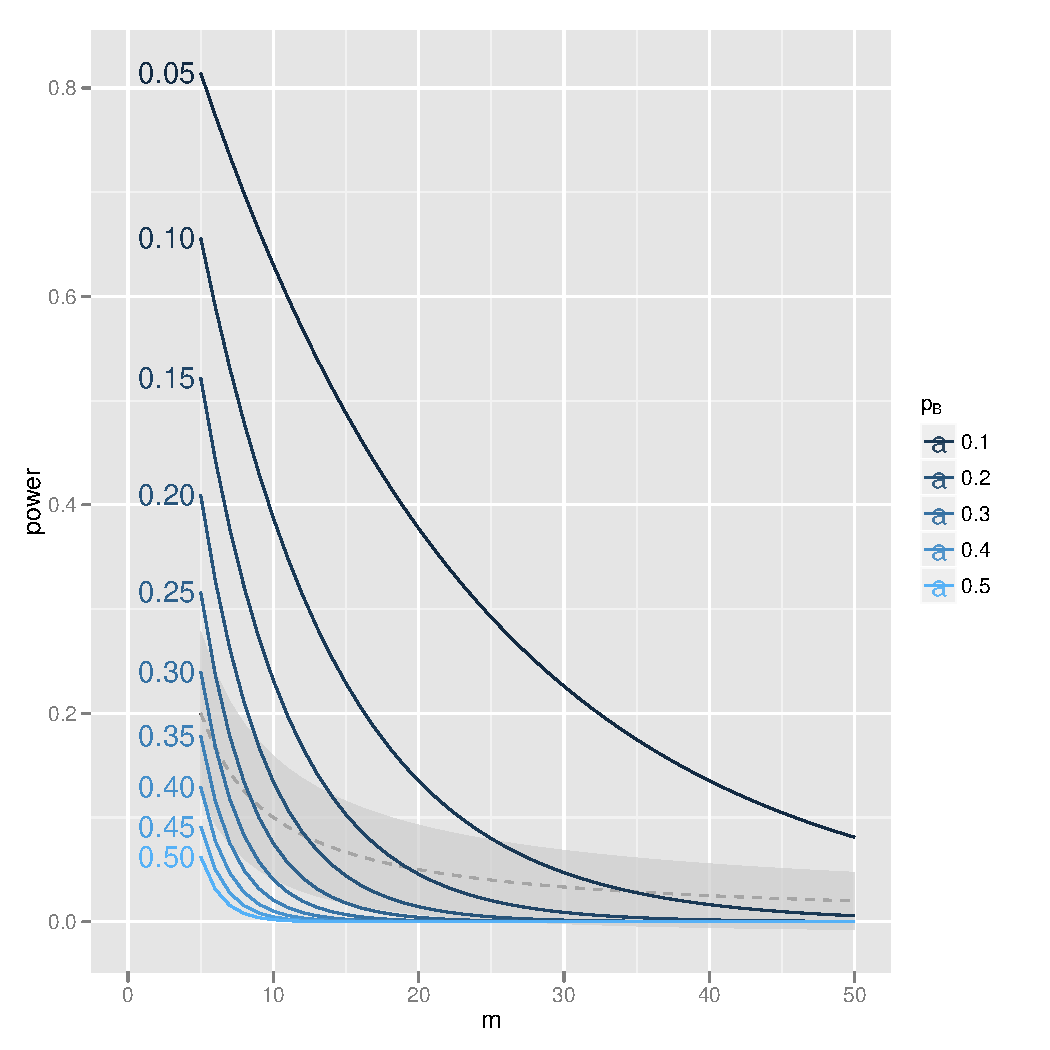
\includegraphics[width=3.8in]{images/powerplot.pdf} 
   \caption{Probability that the data plot has the smallest probability in a lineup of size $m$. With increasing $p$-value the probability drops -- when it reaches $1/m$ a horizontal line is drawn to emphasize insufficient sensitivity of the test due to the lineup size. 
   %Comparison of probabilities to pick the actual data plot for different size lineups, $m$, and different values for data plot strength, $p_D$. The dashed  line, and grey 95\% pointwise confidence band, shows the probability of picking the data plot, by chance, if $H_0$ is true. }
}
   \label{fig:pval_power}
\end{figure}

Now assume that the same lineup plot is evaluated by $K$ independent observers. %W.l.o.g.\green{Can we get rid of cliches like WLOG?} 
Let the last plot be the data plot and plots 1 through $m-1$ the null plots. Let $n_i$ be the number of observers who picked plot $i$ as the plot with the structure least consistent with the null hypothesis, corresponding to random variable $N_i$.  Then  $(N_1, N_2, ..., N_m) \sim$ Mult$_{\pi_1, ..., \pi_m}$ with $\sum_i \pi_i = 1$ and $\sum_{k=1}^{m} n_k = K$. We can estimate $\pi_i$ as $\widehat{\pi_i} = n_i/K$. 

For the distribution of $N_m$, %the number of times out of $K$ that observers picked the last plot to show the structure least consistent with the null hypothesis, 
we get
\[
N_m\sim \left \{ 
\begin{array}{ll}
B_{K, \hh{E\left[ (1 - p_D)^{m-1}\right]}} & \text { under } H_1\\
B_{K, 1/m} & \text { under } H_0
\end{array}
\right .
\]

By matching the expected values, we therefore get an expression for the $p$-value in the data under $H_1$  as:
\begin{equation}\label{eqn:power_estimate}
%{E[p_D]} = 1- \left(\frac{E[N_m]}{K}\right)^{1/(m-1)}.
\hh{1 - E[N_m]/K = (m-1)E[p_D] + O(E[p_D^2])}
\end{equation}

Note that the \hh{left}  hand side in Equation \ref{eqn:power_estimate} is independent of the parameter $\theta$, but just based on the lineup evaluation by independent observers. While this allows us to compute this value independently of the parametric setting, it also means that observers might pick out the data plot for a reason not related to the value of $\theta$. 

%Picking out the data plot is still a measure of how different the data plot is compared to the null plots, and therefore is a test statistic of the visual test.

%This allows us to compute this value independently of the parametric setting. We therefore define the {\it signal strength} of a  visual test as the following:
%
%\begin{dfn} \label{dfn:signal}
%The {\it signal strength} $\sigma_T$ of a visual test is defined as the probability to identify the data plot.
%\end{dfn}
%
%In a lineup of size $m$, evaluated by $K$ independent observers,  we can estimate the signal strength of the test as
%\[
%\sigma_T^{m-1} = \frac{n_m}{K}.
%\]
%
%In a parametric setting, signal strength of a test coincides with the power of the test.



%Theoretical power for the regression parameters is derived in the next section.
%\subsection{Estimating Power from Lineups}
%
%We estimate the empirical power from responses on a specific lineup plot  generated with known values of sample size ($n$), variance ($\sigma^2$) and regression parameter ($\beta$) in model \ref{multi}. Suppose, we have responses from $K$ independent observers with $u$ identifications of the actual plot. This gives an estimated power of
%\begin{equation}\label{power_est} Power(\beta)=\frac{u}{K} \hspace{1cm} 0 \le u \le K \end{equation}


%From model \ref{mixed} we obtain %$\pi=Pr(Y=1|X_1, X_2, ..., X_p)$, 
%the power of the underlying testing procedure as a population average %by ignoring the random effect part. 
%%Thus we have the overall probability of success ($\pi$ or power) 
%for specified sample size ($n$) and  variance ($\sigma$)  as 
%
%\begin{equation}\label{eqn:power} 
%Power(\beta) = \pi=Pr(Y=1|\beta, n, \sigma) 
%\end{equation}
%
%The main covariate factors that determine the power of the test are sample size ($n$), $\sigma$ and the parameter $\beta$. combining these we obtain one single covariate effect denoted by $E$ and defined as $E = \beta/ \sigma*\sqrt{n}$. Using equation \ref{mixed}, we then have the power as
%
%\begin{equation}\label{eqn:effect} 
%Power(E) = \pi=Pr(Y=1| E) 
%\end{equation}

\section{Application to Linear Models} \label{sec:regression}

To make these concepts more concrete consider how this would operate in the linear models setting. Consider a linear regression model 
\begin{equation}\label{multi} Y_i = \beta_0 + \beta_1 X_{i1} + \beta_1 X_{i2} + \beta_3 X_{i1}X_{i2} + ... + \epsilon_i 
\end{equation}
where $\epsilon_i \stackrel{iid}{ \sim } N(0,\sigma^2)$, $i=1,2, .., n$. The covariates ($X_j, j=1,..,p$) can be continuous or discrete.

In this setting, there are many established graphics that are used to evaluate and diagnose the fit of a regression model (e.g. \citet{cook:99}). Table \ref{tbl:stat_multiple} lists several common hypotheses related to the regression setting, and the visual test statistic that might be used for testing these hypotheses. These plots should be familiar, because they are all in common use. For example, to examine the effect of variable $X_j$ on $Y$, we would plot $Y$ against $X_j$ (cases 1-4). To assess whether the linear assumption is appropriate we would make a plot of residuals against fitted values (case 5). For the purposes of comparing visual against classical inference, we focus on cases 2 and 3, with a continuous and catgorical explanatory variable respectively. 

%Note that some charts can be associated with several different testing situations. In our paper, we pick the examples for situation 2 and 3 as candidates.

\begin{table*}[hbtp] 
\caption{Visual test statistics for testing hypotheses related to the model $Y_i = \beta_0 + \beta_1 X_{i1} + \beta_1 X_{i2} + \beta_3 X_{i1}X_{i2} + ... + \epsilon_i  $ } 
\centering 
\begin{tabular}{m{0.5cm}m{3cm}m{2cm}m{3cm}m{5.5cm}} 
\hline\hline 
Case & Null Hypothesis & Statistic & Test Statistic & Description \\ [0.5ex] % inserts table %heading 
\hline 
1 & $H_0: \beta_0=0$ & Scatter plot & \begin{minipage}[t]{3cm}  \scalebox{0.4}{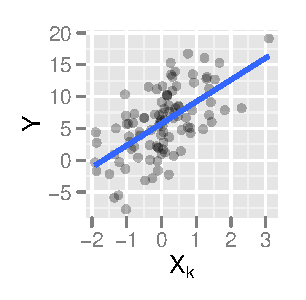
\includegraphics{stat_intercept.pdf}}\end{minipage} & Scatter plot with least square line overlaid. For lineup plot, we simulate data from fitted null model. \\ 
2 & $H_0: \beta_k=0$ & Residual plot & \begin{minipage}[t]{3cm}   \scalebox{0.4}{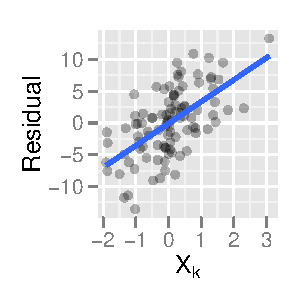
\includegraphics{stat_beta_k.pdf}}\end{minipage} & Residual vs $X_k$ plots. For lineup plot, we simulate data from normal with mean 0 variance $\hat{\sigma}^2$. \\ 
3 & $H_0: \beta_k=0$ (for categorical $X_k$) & Box plot & \begin{minipage}[t]{3cm} 	\scalebox{0.4}{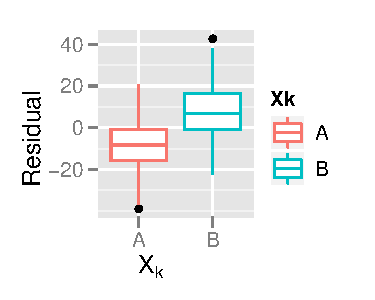
\includegraphics{stat_category.pdf}} \end{minipage} & Box plot of residuals grouped by category of $X_k$. For lineup plot, we simulate data from normal with mean 0 variance $\hat{\sigma}^2$. \\
4 & $H_0: \beta_k=0$ (interaction with categorical $X_k$) & Scatter plot & \begin{minipage}[t]{3cm}  \scalebox{0.4}{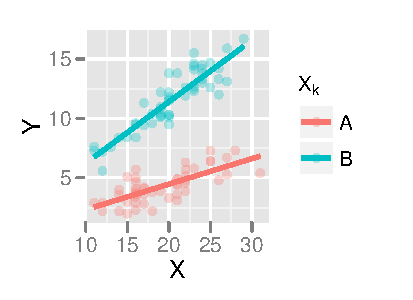
\includegraphics{stat_interection.pdf}}  \end{minipage} & Scatter plot with least square lines of each category overlaid. For lineup plot, we simulate data from fitted null model.\\[1ex] % [1ex] adds vertical space 
5 & $H_0: X$ Linear & Residual Plot & \begin{minipage}[t]{3cm}  	\scalebox{0.4}{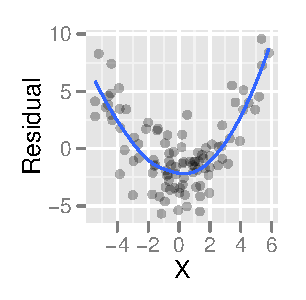
\includegraphics{stat_nonlinear.pdf}}  \end{minipage} & Residual vs predictor plots with loess smoother overlaid. For lineup plot, we simulate residual data from normal with mean 0 variance $\hat{\sigma}^2$. \\ 
6 & $H_0: \sigma^2=\sigma^2_0$ & Box plot & \begin{minipage}[t]{3cm} \scalebox{0.4}{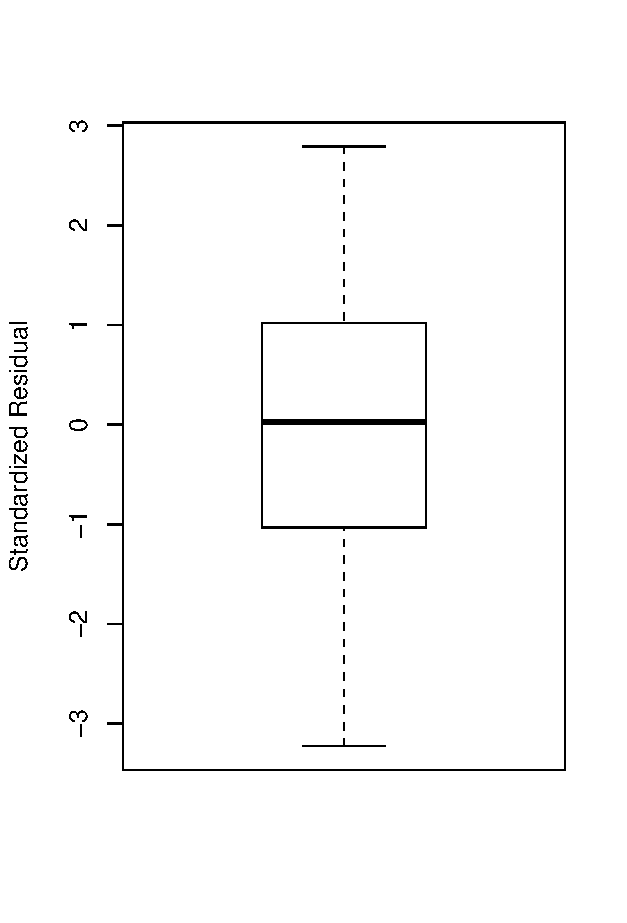
\includegraphics{stat_sigma_box.pdf}}\end{minipage} & Box plot of standardized residual divided by  $\sigma^2_0$. For lineup plot, we simulate data from standard normal. \\ 				
7 & $H_0: \rho_{X,Y|Z}=\rho$ & Scatter Plot & \begin{minipage}[t]{3cm}  	\scalebox{0.4}{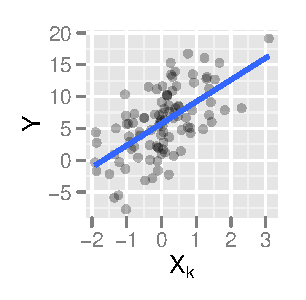
\includegraphics{stat_intercept.pdf}}  \end{minipage} & Scatter plot of Residuals obtained by fitting partial regression. For lineup plot, we simulate data (mean 0 and variance 1) with specific correlation $\rho$. \\ 
8 & $H_0:$ Model Fits & Histogram & \begin{minipage}[t]{3cm}  \scalebox{0.4}{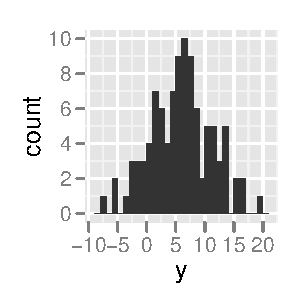
\includegraphics{stat_goodness_simple.pdf}}  \end{minipage} & Histogram of the response data. For lineup plot, we simulate data from fitted model. \\[1ex] % [1ex] adds vertical space 
9 & Special case $p=1$ $H_0: \rho_{X,Y} =\rho$ & Scatter plot & \begin{minipage}[t]{3cm}  \scalebox{0.4}{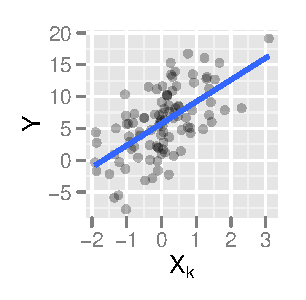
\includegraphics{stat_intercept.pdf}}  \end{minipage} & Scatter plot with least square line overlaid For lineup plot, we simulate data with correlation $\rho$.\\			
\hline 
\end{tabular} 
\label{tbl:stat_multiple} 
\end{table*} 

Suppose $X_k$ is a categorical variable with two levels, and we test the hypothesis $H_0:\beta_k=0$ vs $H_1: \beta_k \ne 0$. If the responses for the two levels of the categorical variable $X_k$ in the model are different and we fit the null model to the actual data, the resulting residuals should show a significant difference between the two groups. To test this boxplots of the residuals conditioned on the two levels of $X_k$ are made, as the observed test statistic. If $\beta_k\ne 0$ the boxplots should show a vertical displacement. 

%A lineup including the test statistic  for a binary $X_k$ is shown in Figure \ref{fig:test_category}. The 19 null plots are generated  by simulating residuals from $N(0,\hat{\sigma}^2)$. The test statistic, the plot containing the actual data, is randomly placed among these null plots. If the test statistic is identifiable the null hypothesis is rejected. % with a $p$-value of at most 0.05.

%\subsection{Expected power}

% Di: This is specific for the regression model
%Consider the hypothesis test $H_0: \beta_k=0$ against $H_1: \beta_k \ne 0$ in model \ref{multi}.
%%Now consider estimating the power of the visual test. 
%%Suppose $F_{|t|}(.)$ is the distribution function of an absolute value of $t$. For the regression slope parameter $\beta$ suppose the associated test statistic in classical test be $t_{obs}$ with $p$-value $p_D$. By definition we have 
%%
%%$$p_D=Pr(|t| \ge t_{obs}| H_0)=1-F_{|t|}(t_{obs}) \Rightarrow |t_{obs}|=F_{|t|}^{-1}(1-p_D)$$
%%
%%\red{HH: the following paragraph should probably move up, but I'm not sure how to change it appropriately. Mahbub, could you take care of that?}
%%Now suppose $F_{|t|}(.;\delta)$ denotes the distribution function of an absolute value of $t$ distribution with non-centrality parameter $\delta$. Thus the distribution function of $p-value$ be  
%%\begin{eqnarray}\label{dist_p}
%%F{p_D}(p) &=& Pr(p_D \le p)=1-Pr(1-p_D \le 1-p) \nonumber \\
%%  &=& 1-Pr(F_{|t|}^{-1}(1-p_D) \le F_{|t|}^{-1}(1-p) ) \nonumber \\
%%  &=& 1-Pr(|t_{obs}| \le F_{|t|}^{-1}(1-p)) \nonumber \\
%%  &=&\left\{ \begin{array}{ll}
%%          1-F_{|t|}( F_{|t|}^{-1}(1-p))=p &\mbox{ ; under $H_0$} \\
%%          1-F_{|t|}( F_{|t|}^{-1}(1-p); \delta) &\mbox{ ; under $H_1$} 
%%       \end{array} \right.     
%%\end{eqnarray}
%%
%%Thus the density of $p_D$ is Uniform(0,1)  under $H_0$. As noted by \cite{Ruppert:2007}, under $H_1$ the density $$f_{p_D}(p_D; \delta)= \frac{f_{|t|}(F_{|t|}^{-1}(1-p_D);\delta)}{f_{|t|}(F_{|t|}^{-1}(1-p_D))}$$ derived from equation \ref{dist_p}  is a right skewed distribution.  
%In a lineup plot we simulate $m-1$ residual data sets from null model where each of these $m-1$ null data sets produces a corresponding $p$-value $p_{0,i}$ and $p_{0,i} \sim \text{Uniform}(0,1)$ for $i = 1, ..., m-1$. Suppose  $p_0=\min_i(p_{0,i})$. Thus $p_0 \sim \text{Beta}(1,m-1)$. 

The conventional test in this scenario uses $T= \hat{\beta_k}/ se(\hat{\beta_k})$ and rejects the null hypothesis if $T$ is extreme on the scale of a $t$ distribution with $n-p$ degrees of freedom.  It forms the benchmark upon which we evaluate the visual test. To calculate what we might expect for the power of the visual test, under perfect conditions, first assume that the observer is able to pick the plot with the smallest $p$-value from a lineup plot.  This leads to the decision to reject $H_0$ when $p_{D} < p_0$, where $p_{D}$ is the classical $p$-value as details given in Lemma \ref{lemma}. Thus the expected power of the visual test in this scenario is

\begin{equation}\label{power_exp} 
   Power(\beta)=Pr(p_{D} < p_0)  \quad \text{for}  \quad \beta \ne 0
\end{equation}
Figure \ref{fig:power_expected} shows the power of the conventional test in comparison to the expected power of the visual test obtained from Equation \ref{power_exp}. Notice that the expected power of the visual test is almost as good as the power of conventional test. \green{What do you mean by this? Where does this ``fact'' come from?} In fact, the only loss we experience stems from comparing the test statistic to only a discrete number of  $m-1$ samples from the null distribution. 

%Theorem \ref{thm:power} helps to compute the expected power of visual inference.
%\begin{thm}\label{thm:power}
% Equation \ref{power_exp}  yields expected power of visual inference as Power($\beta$) = $E(1-p_D)^{m-1}$ .
%\end{thm}
% 
%{ \em proof}
%
%Since $p_0 \sim \text{Beta}(1,m-1)$,  for $t \in (0,1)$ we have the distribution function of $p_0$ be
%\begin{eqnarray*}
%F{p_0}(t) &=& (m-1) \int_0^t{(1-p_0)^{(m-2)}dp_0} \\
%  &=&  -(m-1) \int_1^{1-t}{x^{(m-2)}dx}\\
%  &=& \left[ x^{m-1}\right]^1_{1-t}\\
%  &=&1-(1-t)^{m-1} \rightarrow 1 \quad \text{as} \quad m \rightarrow \infty
%\end{eqnarray*}
%
%% verified this computation from http://www.wolframalpha.com using command int (m-1)*(1-p)^(m-2) dp, p=0,t
%
%Thus expected power in equation \ref{power_exp} be
%\begin{eqnarray*}
% Pr(p_{B} < p_0) &=& 1- Pr( p_0 \le p_{B} ) \\
%  &=& 1- \int_{0}^{1}{Pr( p_0 \le p_{B} |p_{B} =t) f_{p_{B} }(t)dt } \\
%  &=& 1-  \int_{0}^{1}{F{p_0}(t) f_{p_{B} }(t)dt } \\
%  &=& E(1-p_D)^{m-1}   \\
%%  & \rightarrow &1-  \int_{0}^{1}{ f_{p_{B} }(t)dt }  = F_{p_D}(0) \quad \text{as} \quad m \rightarrow \infty
%\end{eqnarray*}
%
%
\begin{figure}[hbtp]
   \centering
       \scalebox{.95}{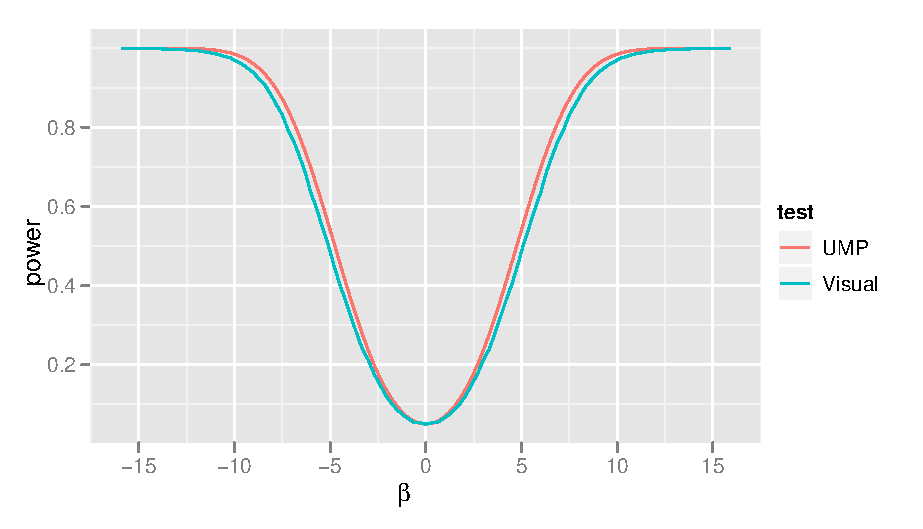
\includegraphics{power_expected.pdf}}
       \caption{Expected power of visual test  and the power of conventional test for sample size $n =100$, $\sigma = 12$ and $m$=20. }
       \label{fig:power_expected}
\end{figure}

% \pagebreak

% -------- Heike's writeup added here

%\subsection{Some Power Considerations}


%\subsection{Expected number of choices}
%Since $X$ has a binomial distribution, we can have a look at the number of plots among the null plots that we would expect to be picked over the data plot:
%\[
%E[X] = (m-1)(1-E[p_D]).
%\]
%With an increase of the lineup size $m$ the number of null plots with a potentially stronger signal than the data plot grows linearly.
%This should allow us to infer some of the signal strength $p_D$ as
%\begin{equation} \label{plot_signal}
%E[p_D] = 1 - E[X]/(m-1),
%\end{equation}
%i.e. by averaging over the number of plots with  a stronger signal than the data plot we can evaluate signal strength of the plot even in the case where the data plot is not being picked by the observer.
%

\section{Human Subjects Experiments with Simulated Data} \label{sec:simulation}

Three experiments were conducted to evaluate the effectiveness of the lineup protocol relative to the equivalent test statistic used in the regression scenario. There are three experiments. The first two are classical settings where we would not expect the lineup protocol to do better than the traditional test, but we hope it to perform favorably. The third experiment is a scenario where assumptions required for the traditional test are violated, and we would expect the lineup protocol to outperform the traditional test. (Data and lineups used in the experiments are available in the supplementary material.)

After many small pilot studies with local personnel, it was clear that some care was needed to set up the human subjects experiments. It was best for a subject to see a block of 10 lineups with varying difficulty, with a reasonable number of ``easy'' lineups. The explanations about each experiment (below) includes an explanation of how the lineups were sampled and provided to the observers, for each of the three experiments.

Participants for all the experiments were recruited through \cite{turk} Amazon's Mechanical Turk. A summary of the data obtained for all three experiments are shown in Table \ref{tbl:summary}. Participants were asked to select the plot they think best matched the question given, provide a reason for their choice, and say how confident they are in their choice. Gender, age, education and geographic location of each participant are also collected. The data was collected through the web. For each of the experiments one of the lineups was used as a test plot (easy plot) which everyone should get correct, so that a measure of the quality of the subjects effort could be made. 

\green{Something probably needs to be said about subjects who do multiple tests, what checks are done.}

\subsection{Discrete covariate}\label{sec:category}

The experiment is designed to study the ability of human observers to detect the effect of a single categorical variable $X_2$ (corresponding to parameter $\beta_2$) in a two variable ($p=2$) regression model (Equation \ref{multi}). Data is simulated a range of values of $\beta_2~ (=0, 1, 3, 5, 7, 8, 10, 16)$, two different sample sizes ($n=100, 300$) and two standard deviations of the error ($\sigma=5, 12$). The range of $\beta_2$ values was chosen so that estimates of the power would produce reasonably continuous power curves, comparable to that calculated for the theoretical conventional test. Values were fixed for other regression parameters, $\beta_0 = 5$,  $\beta_1=15$, and the values for $X_1$ were randomly generated from a Poisson $(\lambda=30)$ distribution, which is almost Gaussian. Data sets were generated with parameter values shown in Table \ref{tbl:experiment_params}. Three replicates at each level were generated. These produced 60 different ``actual data sets'', and thus, 60 different lineups. To produce the lineups, the null model was fit to each actual data set, to obtain residuals and parameter estimates. The actual data plot was generated by making a side-by-side boxplot of the residuals (Table \ref{tbl:stat_multiple}, case 3). The 19 null data sets were generated by simulating from  $N(0, {\hat{\sigma}}^2)$, and these were plotted in the same way as side-by-side boxplots. The actual data plot was randomly placed among these null data plots to produce the lineup. Figure \ref{fig:test_category} is an example of one of these lineups. The actual data plot is number 11 which was generated for $n$=300, $\beta_2$=15 and $\sigma$=12.  

%{\bf Steps to obtain lineup}
%\begin{enumerate}
%	\item For a given parameter setting obtain actual data set
%	\item Fit the null model to the actual data and obtain residuals and other parameter estimates ($\hat{\beta}$ and $\hat{\sigma}$)
%	\item Generate actual data plot using the procedure as described in table \ref{tbl:stat_multiple}
%	\item Generate 19 null (residual) data sets from $N(0, {\hat{\sigma}}^2$) and obtain 19 null plots
%	\item Finally randomly place 19 null plots and one actual plot in a layout (4X5) to get a lineup 
%\end{enumerate}

The number of evaluations required for each lineup to provide reasonable estimates of the power is determined by the variance of the estimated power. Suppose $\gamma$ denotes the conventional test power for each parameter combination shown in table \ref{tbl:experiment_params}. Since the expected power of visual inference is very close to the power of conventional test (Figure \ref{fig:power_expected}) the proportion of successful evaluations of lineups should give a rough estimate for  $\gamma$. For a given proportion $\gamma$ it is desired to have a margin of error (ME) less than or equal to 0.05. Thus we have $ME =1.96 \sqrt{ \frac 1 n_{\gamma} \gamma(1-\gamma)} \le 0.05$ which gives us the estimation of minimum number of evaluations $$n_{\gamma} \geq \frac{\gamma(1-\gamma)}{(0.05/1.96)^2}.$$  

Each subject viewed at least 10 lineups and we allowed them to provide more evaluations if they wanted. Depending on the parameter combinations we group the lineups in different difficulty levels such as easy, medium, hard and mixed (actual numbers are given in the Appendix). For each difficulty level a specific number of lineups were randomly picked to show for evaluation. This number is chosen so that total number of evaluations for each lineup for that group exceed the threshold $n_{\gamma}$. To satisfy this plan we needed to recruit at least 300 subjects. 

\begin{table}[hbtp]
\caption{Combination of parameter values, $\beta_2$,  $n$ and $\sigma$, used for each of the simulation experiments.} % title name of the table
\centering
% centering table
\begin{tabular}{c c c c c}
% creating 10 columns
\hline\hline

% inserting double-line
& & \multicolumn{3}{c}{Slope ($\beta$)} \\
 \cline{3-5}

Sample size  & Error SD  &  \multicolumn{1}{c} {Experiment 1}  & \multicolumn{1}{c} {Experiment 2}  & \multicolumn{1}{c} {Experiment 3} \\
 ($n$) &   ($\sigma$) & Discrete covariate & Continuous covariate & Contaminated data 
\\ [0.5ex]
\hline
% inserts single-line

% Entering 1st row
&  5 & 0, 1,  3, 5, 8  & 0.25, 0.75, 1.25, 1.75, 2.75 & 0.1, 0.4, 0.75, 1.25, 1.5, 2.25\\[-1ex]
\raisebox{1.5ex}{100} &12
& 1, 3, 8, 10, 16  & 0.5, 1.5, 3.5, 4.5, 6 &\\[1ex]

% Entering 2rd row
&  5 & 0, 1, 2, 3, 5  & 0.1, 0.4, 0.7, 1, 1.5&\\[-1ex]
\raisebox{1.5ex}{300} & 12
& 1, 3, 5, 7, 10  & 0, 0.8, 1.75, 2.3, 3.5 &\\[1ex]
% [1ex] adds vertical space
\hline
% inserts single-line
\end{tabular}
\label{tbl:experiment_params}
\end{table} 

%For a given proportion $p$ we want to have margin of error (ME) to be 0.1. Thus we have $ME =1.96 \sqrt{ \frac 1 n p(1-p)} \le 0.05$ which gives us the estimation of minimum number of evaluations $$n_p \geq \frac{p(1-p)}{(0.05/1.96)^2}.$$ Now from the theoretical (UMP) power curve for each parameter combinations shown in table \ref{tbl:experiment_params} we know the power(say $p$) and thus we can estimate the number of evaluations required for that specific combinations of parameter. We collect data such that each of the parameter combinations in the table \ref{tbl:experiment_params} has approximately the estimated sample size that we calculated here.
 


%\green{Did you in fact bin like this???}\red{For each parameter combination a set of 1000 actual data are generated and their associated p-values were computed. This produces an empirical distribution of p-value under alternative hypothesis. Finally, three data sets that have 16th, 50th and 84th quantile of the p-values were taken. Similar procedure was used to generate 19 null plots based on the empirical distribution of p-value under null hypothesis}. For added control, to ensure a signal in the simulated actual data a blocking structure was used to filter data sets. A 1000 sets were generated for each parameter combination and the traditional $t$-statistic and $p$-value associated with $H_0: \beta_2=0$ were calculated. The 3 replicates were drawn from each of three blocks of $p$-values: (0.0-$q_{33}$), ($q_{33}$-$q_{66}$), ($q_{66}$-1) where $q_i$ is the $i$th percentile in the distribution of the $p$-values. Additional control was applied to the 19 null plots. Because the distribution of these $p$-values should follow a Uniform(0,1) distribution, data sets were binned on this range by $p$-value, and a data set was randomly selected from each bin.
  
\subsection{Continuous covariate} 

This experiment is very similar to the previous one, except that there is a single continuous covariate and no second covariate (Equation \ref{multi} with $p=1$), following the test in Table \ref{tbl:stat_multiple}, case 2. Data is simulated with two sample sizes ($n=100, 300$), two standard deviations of the error ($\sigma=5, 12$), a variety of slopes ($\beta$), as given in Table  \ref{tbl:experiment_params}. We arbitrarily fix $\beta_0 = 6$ and values for $X_1$ are simulated from $N(0,1)$. For each combination of parameters, three different actual data sets are produced, yielding a total of 65 lineups. For some parameter combinations we have more than three replications, because additional lineups were produced for values of the parameters that exhibited large variation in the initial data.

The actual data plot is generated by making a scatterplot of $Y$ vs $X_1$ with the least squares regression line overlaid. To produce the null plots in the lineup null data was simulated from $N(X \hat{\beta}, {\hat{\sigma}}^2$) and plotted using the same scatterplot method as the actual data. 
An example lineup from this experiment is shown in Figure \ref{fig:test_continuous}.  This lineup is generated using sample size ($n$)=100, slope($\beta$)=1.25 and and error SD($\sigma$)=5. The actual data plot location is 11. This lineup, we think, is a difficult one. To select 10 lineups for a subject, each combination of sample size ($n$) and error SD ($\sigma$) is given a difficulty value based on the slope ($\beta$) parameters. For the smallest slopes the difficulty is 4 (hardest) and for the largest slopes the difficulty is 0 (easiest). For one combination of sample size and standard deviation, the subject sees a randomly selected lineup of each difficulty level, all the slopes, giving 5 lineups. Another four lineups are chosen from a second choice of sample size and standard deviation, with difficulty levels 0-3, and the last lineup shown was a randomly selected lineup with difficulty 0. The order that the lineups are shown to participants is randomized. Each subject saw a substantial number of difficult lineups. \hh{While this allows us a better estimation for the power in small slopes, }
%The intention was noble, to get a better handle on the power of the lineups for small slopes, 
but practically this made the study very tiring for the participants. %It would be better to provide the subjects with a larger selection of easier lineups and just a few difficult ones. 
\green{perhaps should go into so much detail about this, or keep this for the conclusions section.}  

%{\bf Steps to obtain lineup}
%\begin{enumerate}
%	\item For a given parameter setting obtain actual data set
%	\item Fit the null model to the actual data and obtain residuals and other parameter estimates ($\hat{\beta}$ and $\hat{\sigma}$)
%	\item Generate actual data plot (a scatter plot of $Y$ vs $X_1$ a least square line overlaid)
%	\item Generate 19 null data sets from $N(X \hat{\beta}, {\hat{\sigma}}^2$) and obtain 19 null plots
%	\item Finally randomly place 19 null plots and one actual plot in a layout (4X5) to get a lineup 
%\end{enumerate}

%\green{Fill in details of lineups, probably need a figure with an example lineup, and how lineups were assigned to subjects.}

%{\bf Presenting lineups for evaluation} Each subject got at least 10 lineups for evaluation. For each combination of sample size ($n$) and error SD ($\sigma$) we define the difficulty of the lineup based on the five slope ($\beta$) parameters we choose as shown in table \ref{tbl:experiment_params}. For the smallest slope parameter the difficulty is 0 and for the largest parameter the difficulty is 4. The 10 lineups are chosen as follows;

%\begin{enumerate}
%	\item For one combination of  sample size ($n$) and error SD ($\sigma$) randomly select five lineups with one from each difficulty level
%	\item For another combination of sample size ($n$) and error SD ($\sigma$) select four lineups with one from each difficulty level 0 through 3
%	\item Finally select another lineup with difficulty level 0
%\end{enumerate}


\begin{figure}[htp]
%\begin{figurehere}
   \centering
       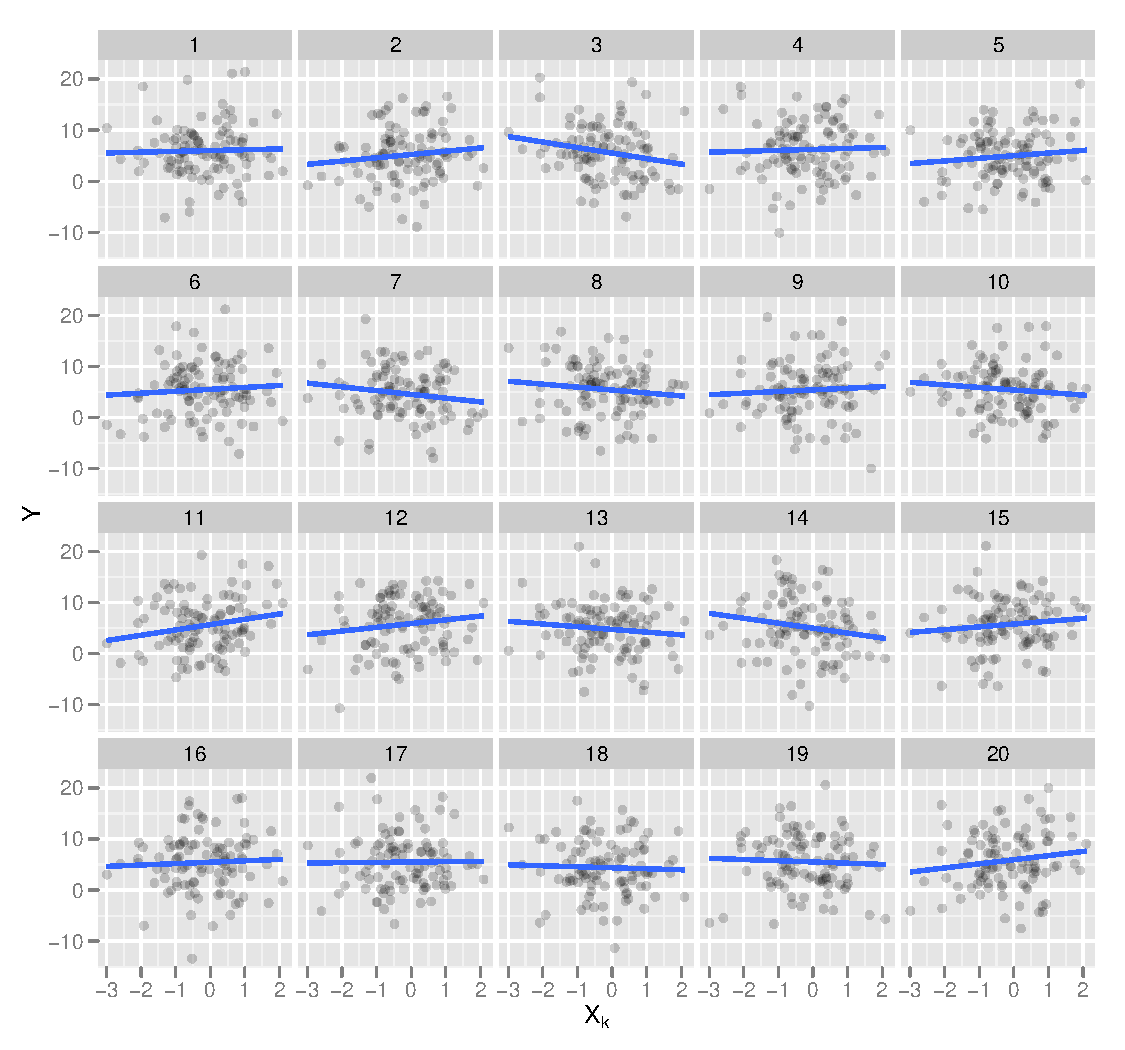
\includegraphics[width=0.95\textwidth]{lineup_continuous.pdf}
       \caption{Lineup plot ($m=20$) using scatter plots for testing $H_0: \beta_k=0$ where covariate $X_k$ is continuous. One of these plots is the plot of the actual data, and the remaining are null plots, produced by simulating data from a null model that assumes $H_0$ is true. Which plot is the most different from the others, in the sense that there is the steepest slope?}
       \label{fig:test_continuous}
\end{figure}

\subsection{Contaminated data}

The first two simulation experiments use data generated with a normal error model, satisfying the conditions for conventional test procedures. In these situations there exists a test, and there would, in general, be no need to use visual inference. The simulation is conducted with the hopes that the visual test procedure, although not expected to beat the conventional test, will compare favorably with it. This third simulation is closer to the mark for the purpose of visual inference. The assumptions for the conventional test are violated, by contaminating the data. The contamination makes the estimated slopes effectively 0, yet the true value of slope parameter is not.  The data is generated from the following model:

\[
  Y_i = \left\{
  \begin{array}{l l}
    \alpha+\beta X_i + \epsilon_i  & \quad  X_i \sim N(0,1) \quad  i =1,...,n\\
    \lambda+ \eta_i & \quad X_i \sim N(\mu,1/3) \quad  i=n+1, ...,n*c\\
  \end{array} \right.
\]
where $\epsilon_i \stackrel{iid}\sim N(0,\sigma)$, $\eta_i \stackrel{iid}\sim N(0,\sigma/3)$ and $\mu = -1.75$, $c$ is the proportion of contaminated data. For the experiment we consider $n=100$, $c=0.15$ producing actual data with $115$ points. Also $\alpha=0$ and $\lambda=10$, and $\sigma$ is chosen to be approximately 3.5, so that error standard deviation across both groups of the data is $5$. Figure \ref{fig:cont_dat} shows an example of contaminated data, generated by this model for $\beta=5$.  A linear model (Equation \ref{multi} with $p=1$  and intercept $\beta_0=0$) is fit to the contaminated data. This experiment also follows the test in Table \ref{tbl:stat_multiple}, case 2. The actual data plot shows a scatterplot of the residuals vs $X_1$, and the null data plots are scatterplots of null data generated by simulating residuals from $N(0, {\hat{\sigma}}^2$) and plotting against $X_1$. 

Five replications of actual data sets for each slope value shown in Table \ref{tbl:experiment_params}, producing 30 lineups. Six groups of difficulty level based on slope are defined, difficulty = 0 for largest slope and difficulty = 5 for the smallest slope.    Eight (8) lineups with two from each of the difficulty group from 0 through 3 and two(2) lineups with one from each difficulty group 4 and 5 were randomly picked for each subject. 

%{\bf Steps to obtain lineup}
%\begin{enumerate}
%	\item For a given parameter setting obtain actual data set
%	\item Fit the null model to the actual data and obtain residuals and other parameter estimates ($\hat{\beta}$ and $\hat{\sigma}$)
%	\item Generate actual data plot (a scatter plot of Residual vs $X_1$)
%	\item Generate 19 null residual data sets from $N(0, {\hat{\sigma}}^2$) and obtain 19 null plots
%	\item Finally randomly place 19 null plots and one actual plot in a layout (4X5) to get a lineup 
%\end{enumerate}

An example lineup for slope $\beta=0.4$ is shown in Figure \ref{fig:test_contaminated}.  Can you pick which plot is different? %Plot 7 is the actual data plot. 
\begin{figure}[hbt]
%\begin{figurehere}
   \centering
       \scalebox{0.4}{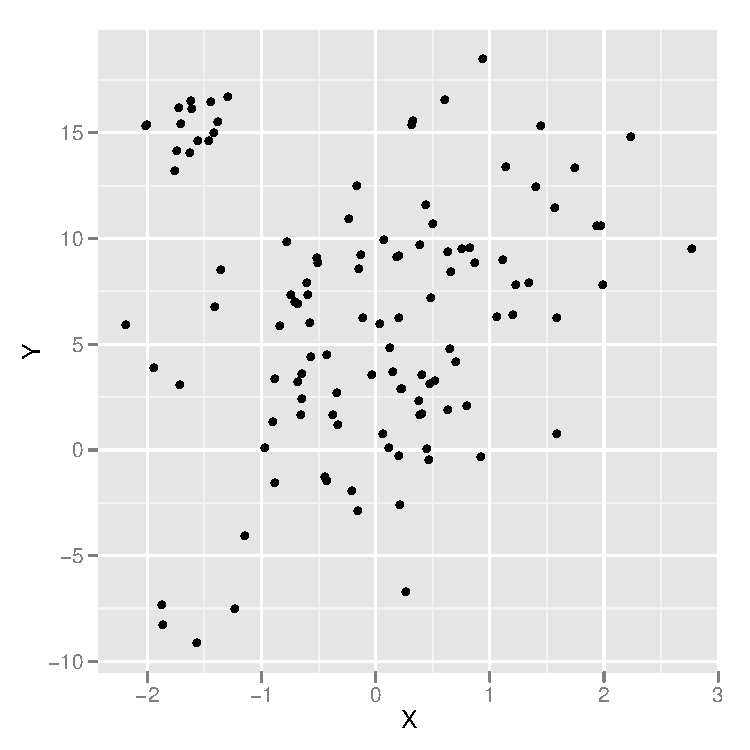
\includegraphics{contaminated_data.pdf}}
       \caption{Scatterplot of a simulated contaminated data set generated such that a simple linear model produce a slope almost negligible, ie, if we fit model (Equation \ref{multi}) with $p=1$  to this data, the resulting estimate of $\beta_1$ would not be statistically significant.
}
       \label{fig:cont_dat}
\end{figure}

\begin{figure}[htp]
%\begin{figurehere}
   \centering
       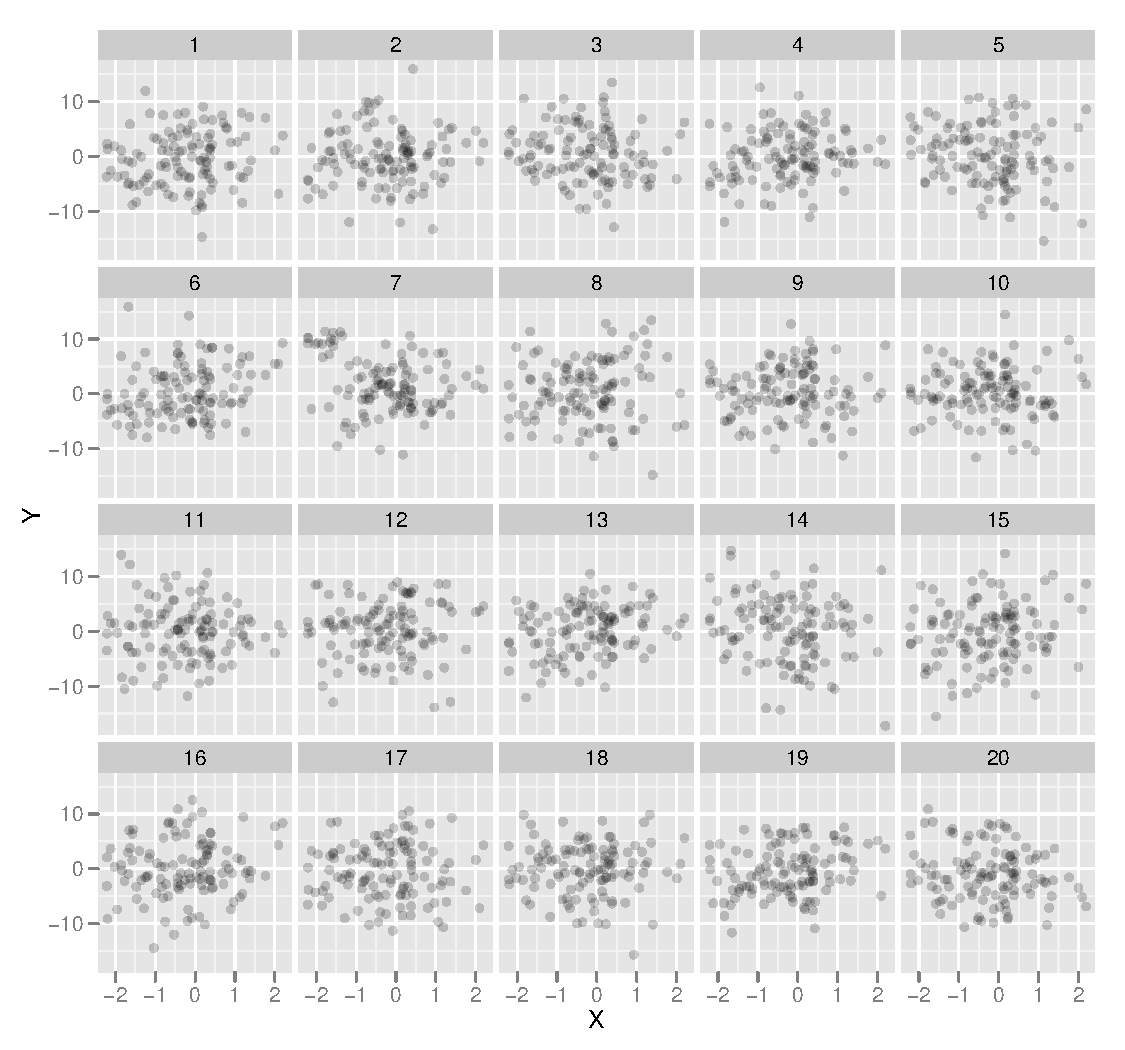
\includegraphics[width=0.95\textwidth]{lineup_contaminated.pdf}
       \caption{Lineup plot ($m=20$) using scatter plots for testing $H_0: \beta_k=0$ where covariate $X_k$ is continuous but the inclusion of some contamination with the data spoils the normality assumption of error structure. One of these plots is the plot of the actual data, and the remaining are null plots, produced by simulating data from a null model that assumes $H_0$ is true. Which plot is the most different from the others, in the sense that there is the steepest slope?}
       \label{fig:test_contaminated}
\end{figure}

%\green{Fill in details of lineups, probably need a figure with an example lineup, and how lineups were assigned to subjects. Show a sample lineup, probably the most difficult, instead of the single plot.}


%\begin{figure*}[hbtp]
%   \centering
%       \scalebox{0.6}{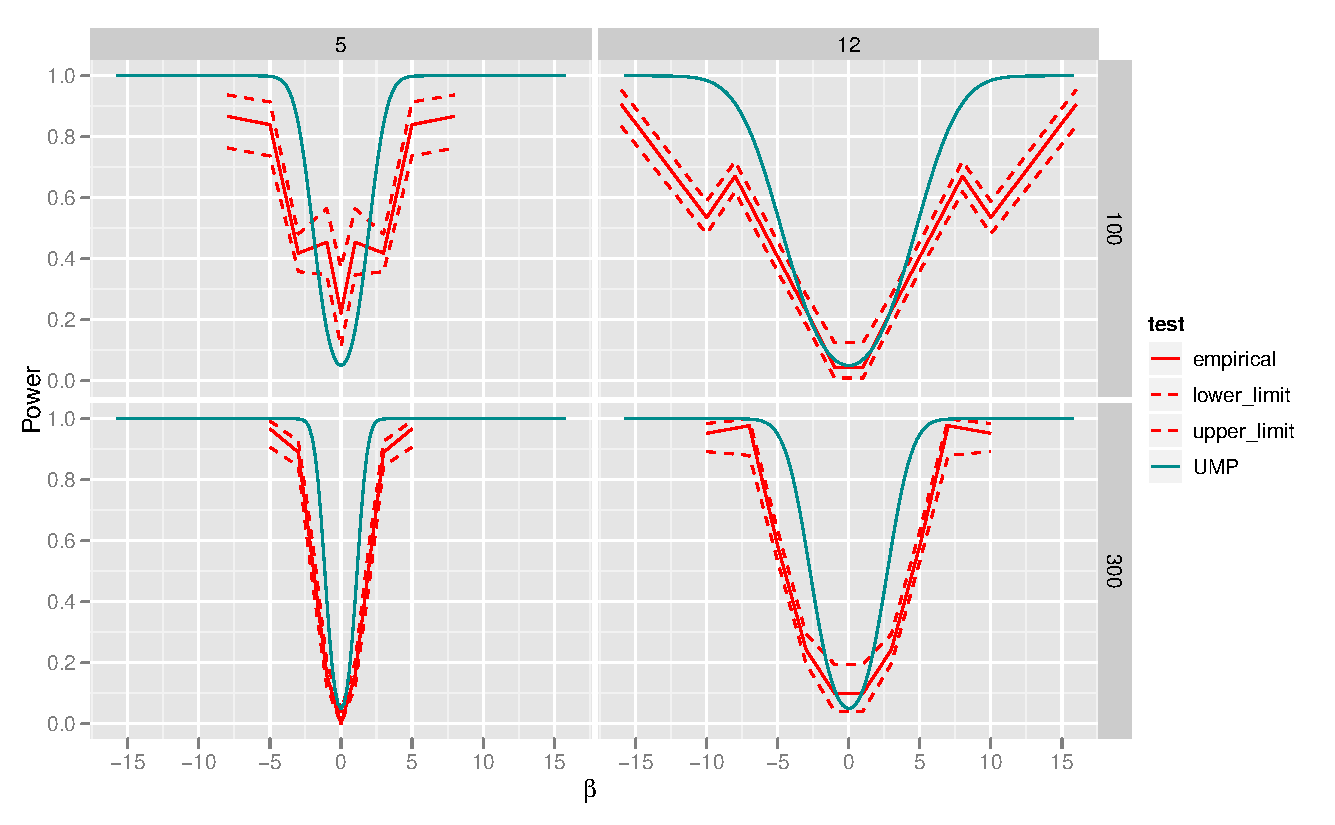
\includegraphics{power_observed.pdf}}
%       \caption{Observed power of visual test from Equation \ref{eqn:power_estimate} with pointwise 95\% confidence limits and the power of UMP test for sample size $n= 100,300$ and $\sigma = 12,5$ as per experiment 1.}
%       \label{fig:power_observed}
%\end{figure*}

%\begin{figure*}[hbtp]
%   \centering
%       \scalebox{0.7}{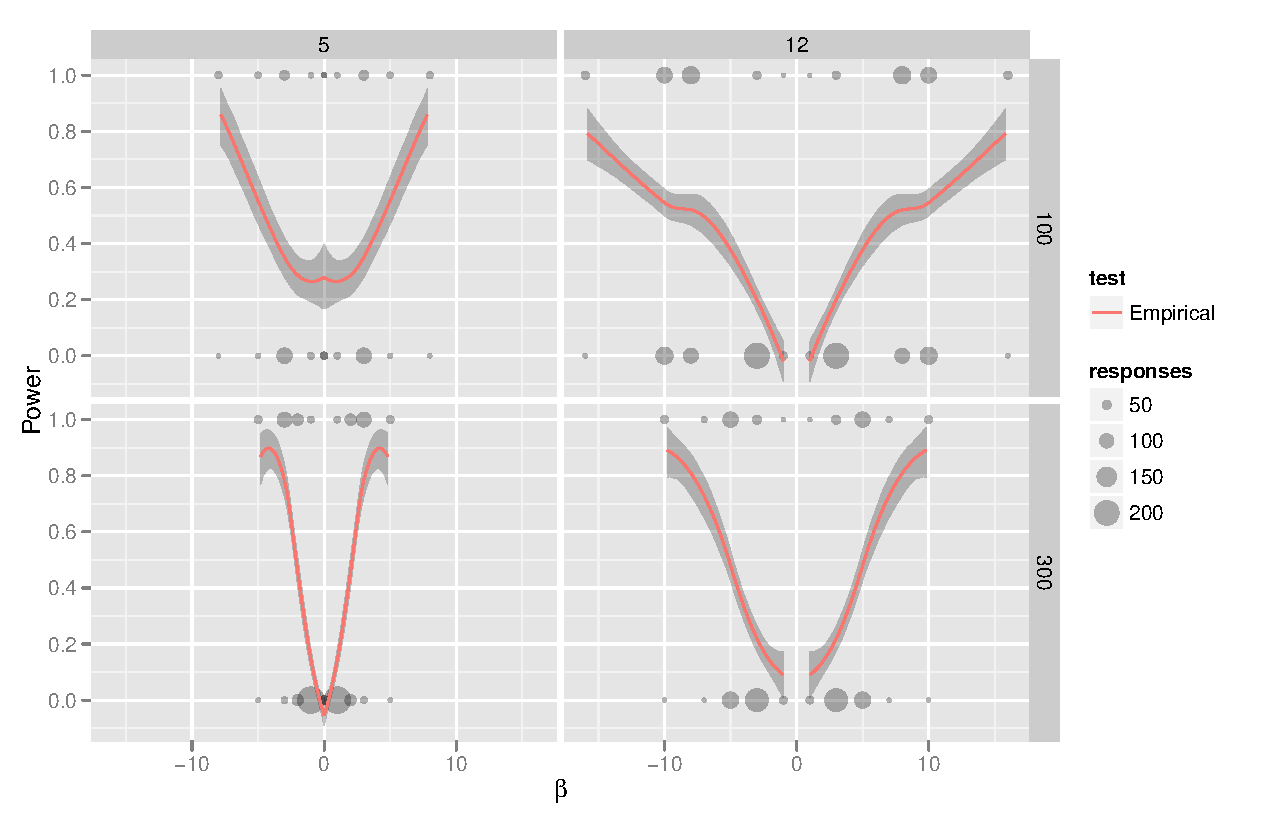
\includegraphics{power_loess_exp1.pdf}}
%       \caption{Observed power shown by loess smoother with simultaneous bootstrap confidence band and the power of UMP test for sample size $n= 100,300$ and $\sigma = 12,5$ as per experiment 1.}
%       \label{fig:power_loess1}
%\end{figure*}


%\begin{figure*}[hbtp]
%   \centering
%       \scalebox{0.7}{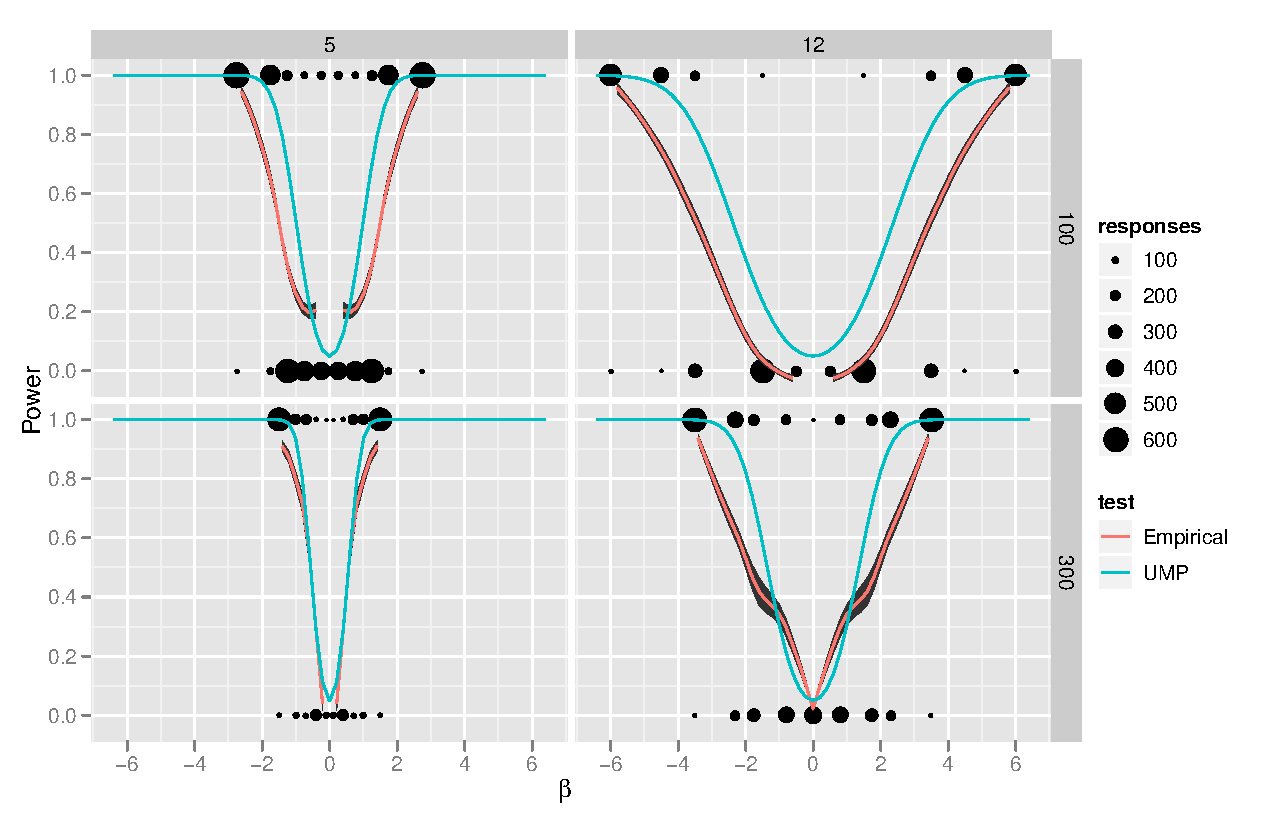
\includegraphics{power_loess_exp2.pdf}}
%       \caption{Observed power shown by loess smoother with simultaneous bootstrap confidence band and the power of UMP test for sample size $n= 100,300$ and $\sigma = 12,5$ as per experiment 2.}
%       \label{fig:power_loess2}
%\end{figure*}




%\begin{figure*}[hbtp]
%   \centering
%       \scalebox{0.7}{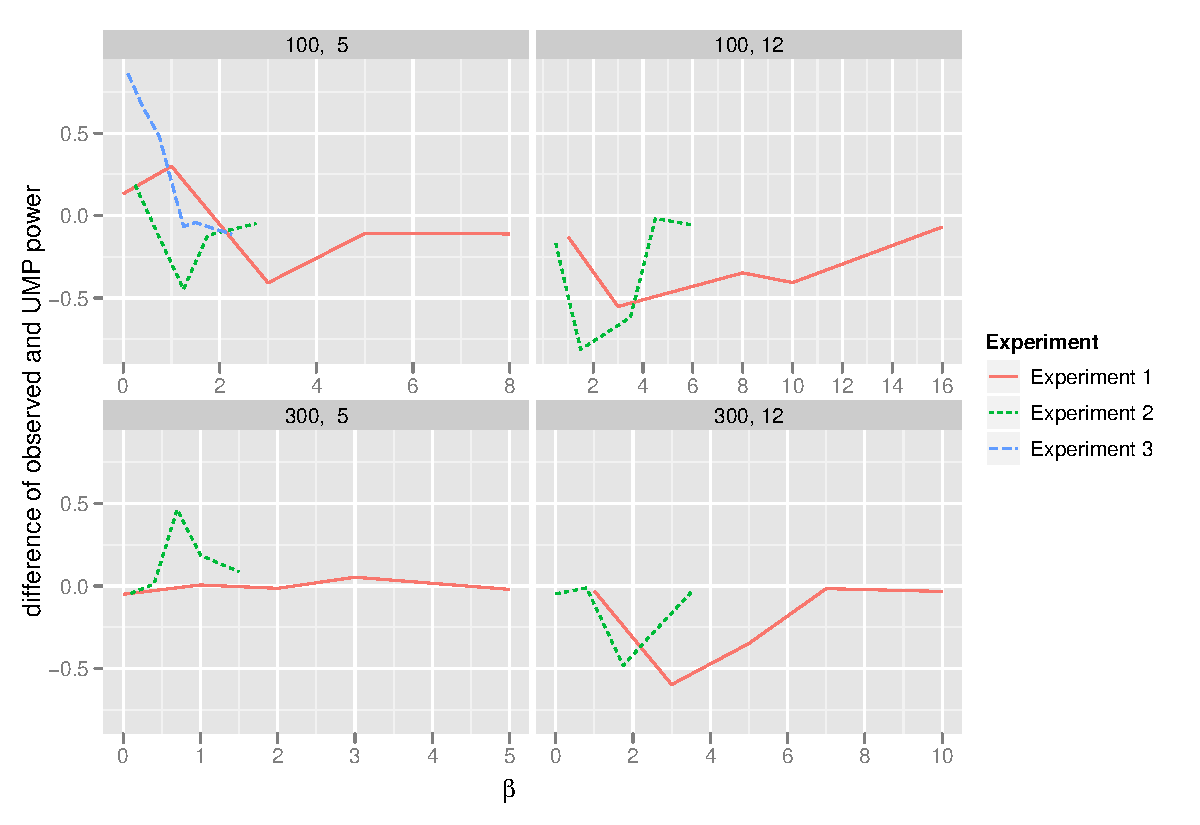
\includegraphics{power_diff_exp.pdf}}
%       \caption{Difference of Observed power from UMP test power obtained in three experiments for sample size $n= 100,300$ and $\sigma = 12,5$ and values of slope parameter $\beta$ as shown in table \ref{tbl:experiment_params}.}
%       \label{fig:power_diff_exp}
%\end{figure*}


%\begin{figure*}[hbtp]
%   \centering
%       \scalebox{0.6}{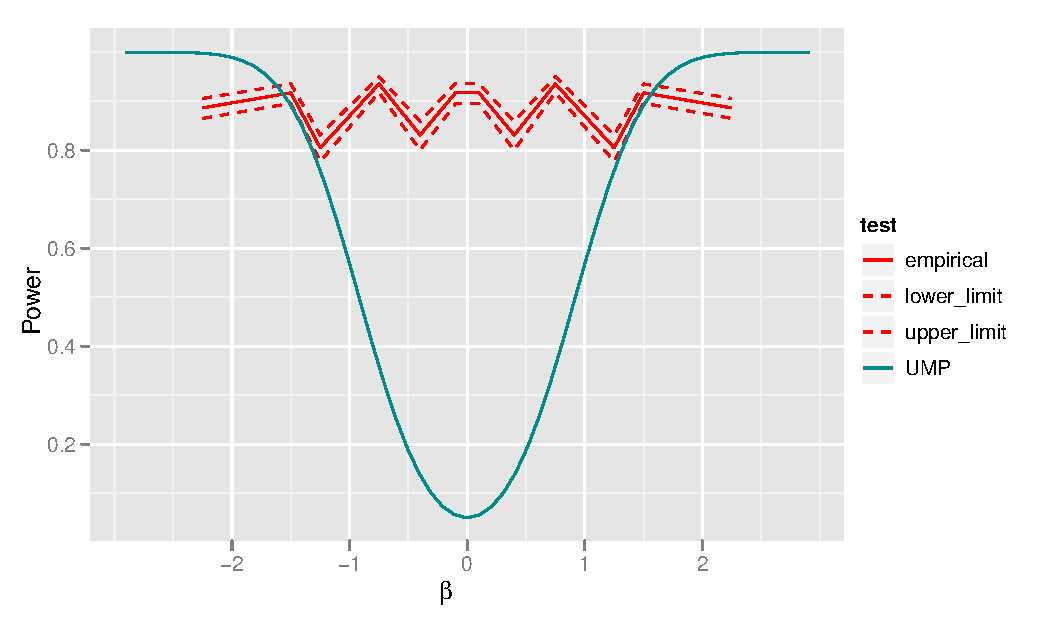
\includegraphics{power_observed_exp3.pdf}}
%       \caption{Observed power of visual test from Equation \ref{eqn:power_estimate} with pointwise 95\% confidence limits and the power of UMP test for sample size $n= 100$ and $\sigma = 5$ as per experiment 3. }
%       \label{fig:power_observed_exp3}
%\end{figure*}


\section{Results}

\subsection{Data Screening}

% In this process of collecting data some participants did not provide demographic information as we see in Table \ref{tbl:summary} that male and female participants do not add up to total participants. It is not clear why they did not provide the information. Now the concern arises whether we should keep their responses in the study. It is also possible that participants were not serious enough to provide feedback. 
%For each of the experiments we had a test plot (easy plot) for which they should have a correct evaluation without much effort.  This could be a criteria to determine their attentiveness in the study. For this we consider six different data cleaning criteria as shown below;

{\bf Screening scenarios:} \hh{Amazon Mechanical Turk data often suffers from the problem that some participants are trying to 'game' the system -- in our situation, these are participants who did not put in a best effort to identify the data plot, but just randomly picked a plot to maximize their 'winnings'.  In order to avoid using those results, we are comparing six different screening methods for excluded participants from the data analysis.} 
%There are six suggested approach to clean the data. 
They are 
\begin{enumerate}
\item {\bf include all participants} and their evaluations
\item exclude all participants' evaluations, who did {\bf not} share their {\bf demographic information} (age, gender education level -- all three pieces of information are either missing or all present).
\item exclude participants' records, if {\bf none of the evaluations}  correctly identified the data plot -- every participant was shown a range of `easy' lineups.
\item include participants' records, if   {\bf at least 20 percent} of the evaluations are {\bf correct}  -- based on ten evaluations per participants, two correct evaluations are significant evidence against a person just guessing
\item include participants' records, if at least {\bf 50\% of all very easy lineups are correct} 
\item use easy lineups as {\bf reference charts}: sample one easy lineup from a person's records. If that lineup is evaluated {\bf correctly}, include all (other) lineups of that person, otherwise exclude all lineup evaluations by this participant.
\end{enumerate}

\begin{table}[hbtp]
\caption{Number of unique subjects and their total feedbacks after applying six screening process on all three experimental data sets. 
Note that in some of the lines the number of male and female participants does not add up to the total number of participants. This is due to missing demographic information. \hh{Do we need this table or could we make this a visual comparison? For me, there's too many numbers with too many digits.}}
\begin{center}
\begin{tabular}{rrrrr|rrrr|rrrr}
  \hline
Screening &  \multicolumn{4}{c} {Experiment 1}  & \multicolumn{4}{c} {Experiment 2}  & \multicolumn{4}{c} {Experiment 3} \\
 \cline{2-5}  \cline{6-9}   \cline{10-13}
criteria & Subj & Male & Fem & Total & Subj & Male & Fem & Total & Subj & Male & Fem & Total \\ 
  \hline
1 & 520 & 264 & 201 & 4914 & 390 & 203 & 182 & 4603 & 257 & 166 &  84 & 2830 \\ 
  2 & 465 & 264 & 201 & 4624 & 385 & 203 & 182 & 4558 & 250 & 166 &  84 & 2782 \\ 
  3 & 384 & 200 & 165 & 4187 & 384 & 199 & 181 & 4573 & 227 & 147 &  78 & 2648 \\ 
  4 & 318 & 168 & 135 & 3395 & 378 & 195 & 179 & 4492 & 205 & 133 &  72 & 2393 \\ 
  5 & 277 & 139 & 124 & 3008 & 374 & 193 & 177 & 4451 & 112 &  73 &  39 & 1410 \\ 
  6 & 239 & 121 & 107 & 2317 & 351 & 185 & 164 & 3858 &  98 &  64 &  34 & 1095 \\ 
   \hline
\end{tabular}
\end{center}
\label{tbl:summary}
\end{table}



\subsection{Power comparison}

We fit model \ref{mixed} with effect $E=\beta*n/\sqrt(n)$ as the only fixed effect covariate without intercept. We also set $offset = log(0.05/95)$ so that the estimated power has a fixed lower limit = 0.05 (Type-I error) for effect $E=0$. The power curves obtained by fitting model \ref{mixed} to the data for all the experiments applying different screening criteria is shown in figure \ref{fig:power_screening}. This shows how the screening criteria may affect the results. The corresponding power curves of conventional test are also shown. Notice that no mater what criteria we apply the result does not change much for experiment 2. Also, estimated power curve with criteria 5 for experiment 3 is above the conventional test power curve.

\begin{figure}[hbtp]
   \centering
       \scalebox{0.70}{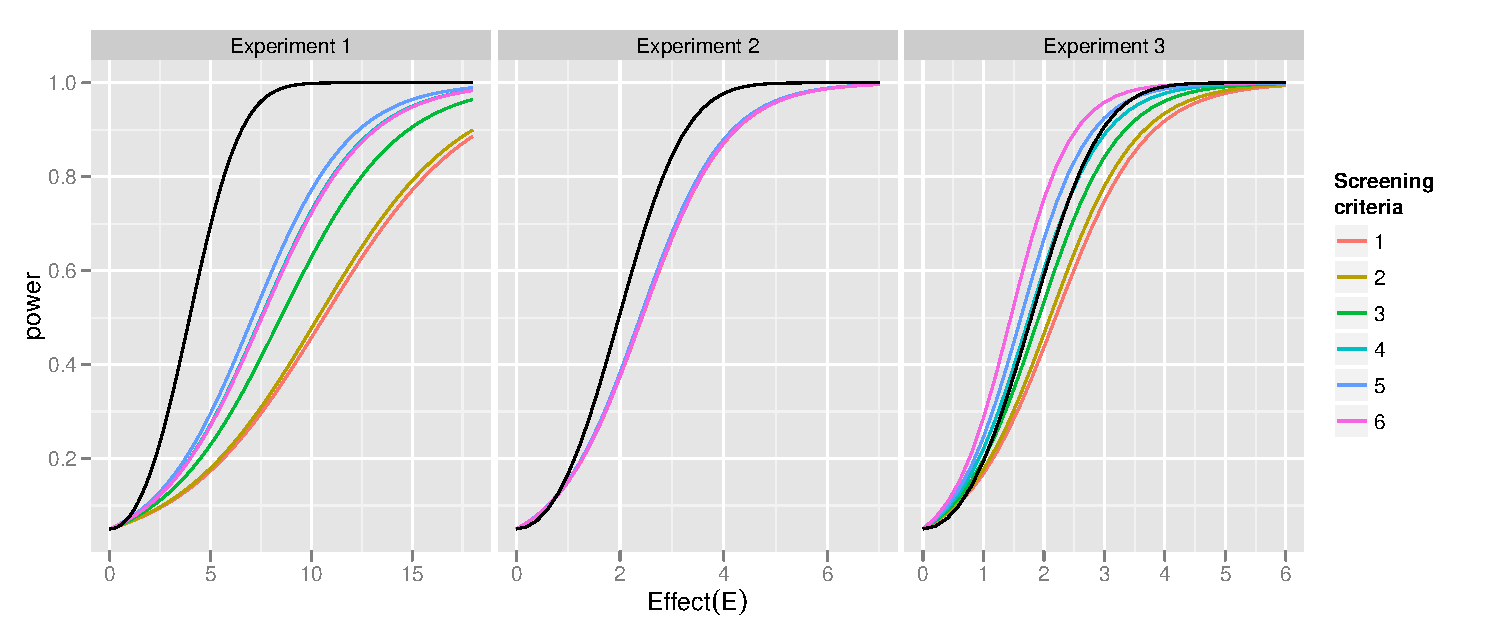
\includegraphics{power_screening.pdf}}
       \caption{The overall power estimated from model \ref{mixed} are shown for various data sets obtained by applying 6 screening criteria.  The corresponding power curve for conventional test is shown in black solid lines for comparison.}
       \label{fig:power_screening}
\end{figure}




%Each participant was shown a sequence of 10 lineup plots.  In total, 3629 lineups were evaluated by 324 people coming from many different locations across the globe.  The results of the experiment are summarized in Figure \ref{fig:power_observed} which shows the observed power from the survey data calculated using Equation \ref{eqn:power_estimate} along with 95\% confidence interval calculated using Fisher's exact method.

\begin{figure*}[hbtp]
   \centering
       \scalebox{0.45}{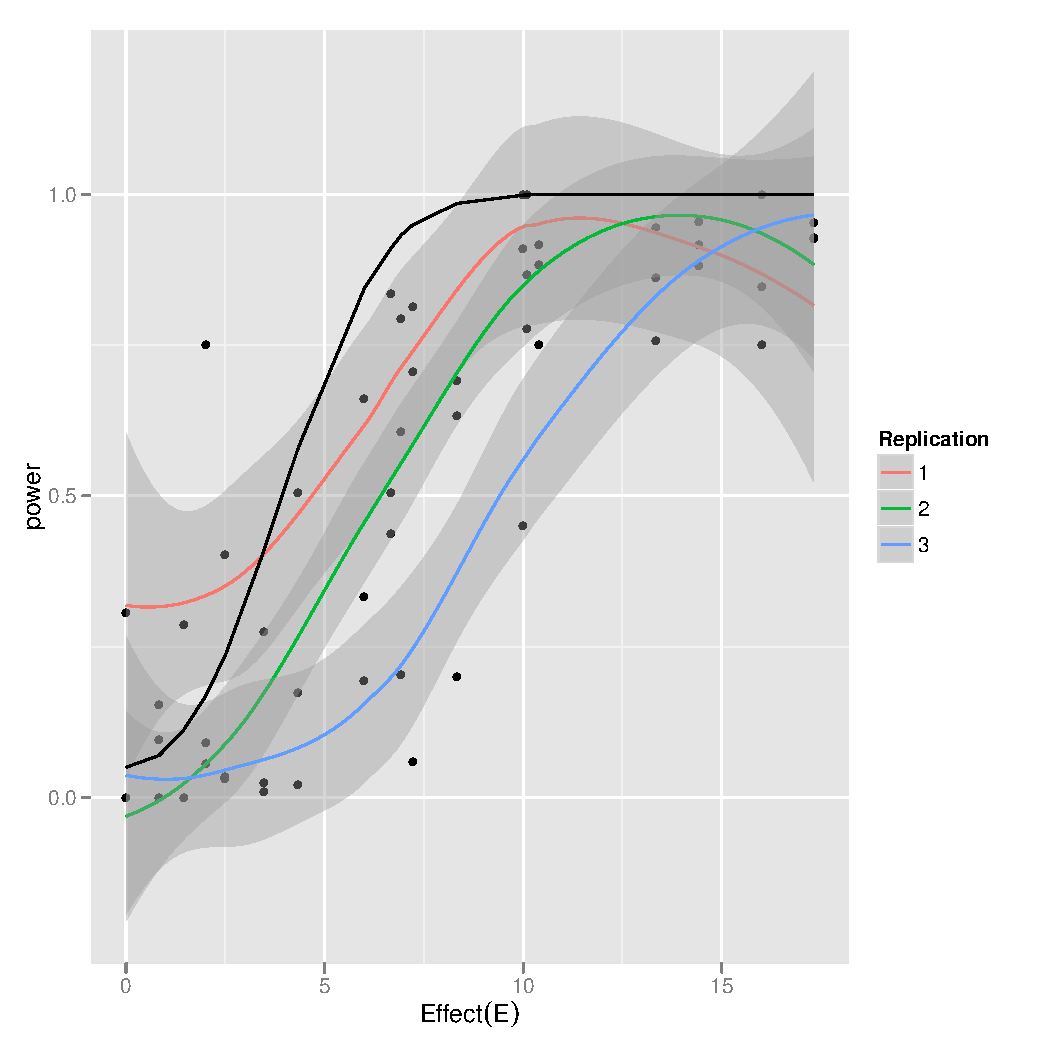
\includegraphics{effect_power_exp1.pdf}}
       \scalebox{0.45}{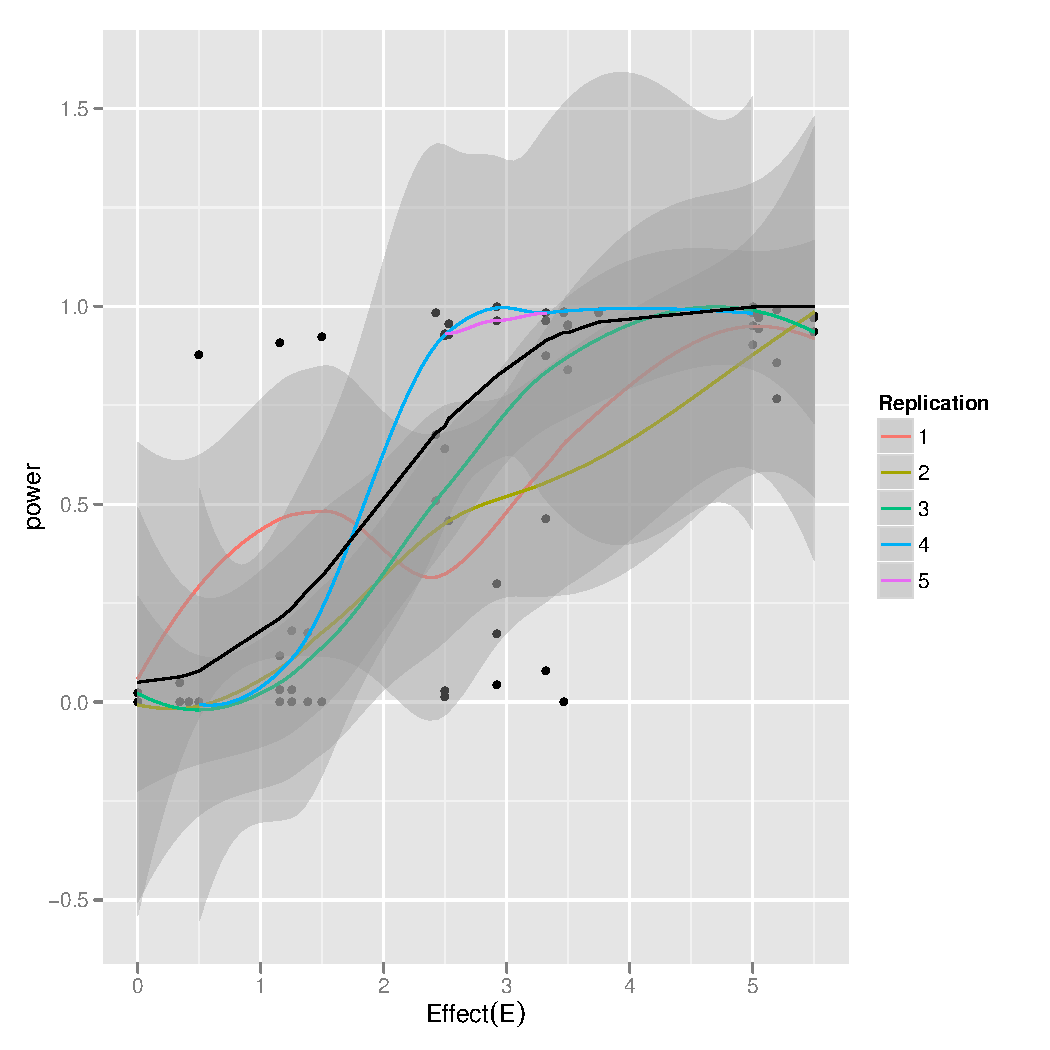
\includegraphics{effect_power_exp2.pdf}}
       \caption{Observed power shown by loess smoother and the power of conventional test for different effect size $E$ as per experiment 1 and 2.}
       \label{fig:power_effect1}
\end{figure*}

%\begin{figure*}[hbtp]
%   \centering
%       \scalebox{0.45}{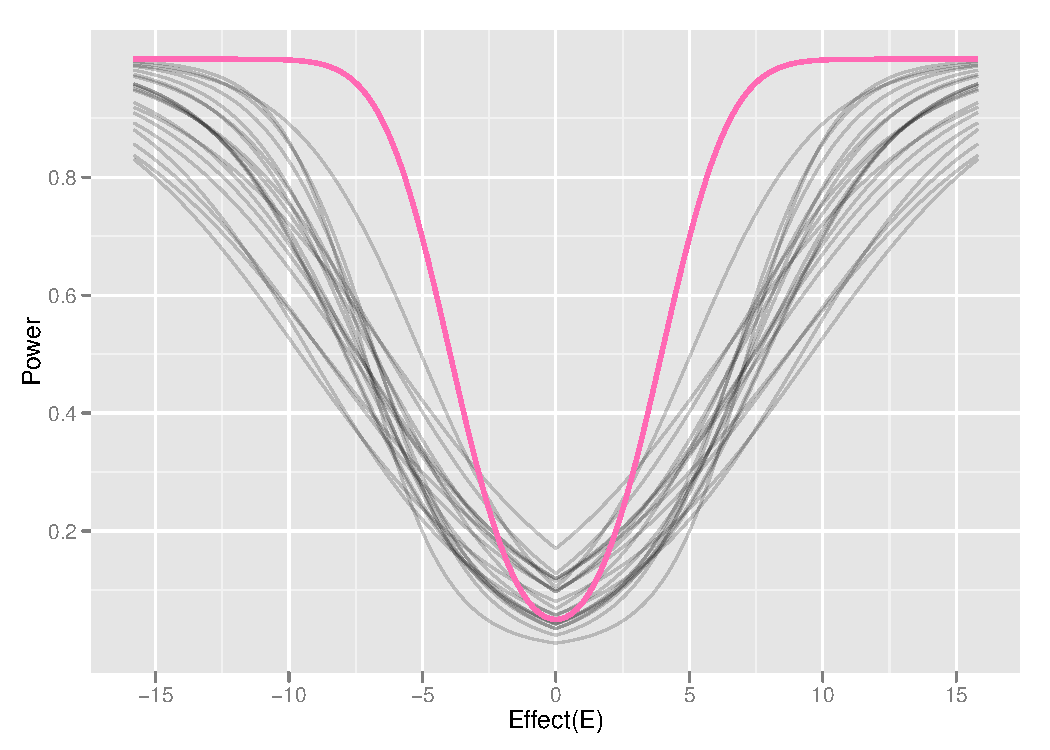
\includegraphics{effect_power_subject_exp1.pdf}}
%       \scalebox{0.45}{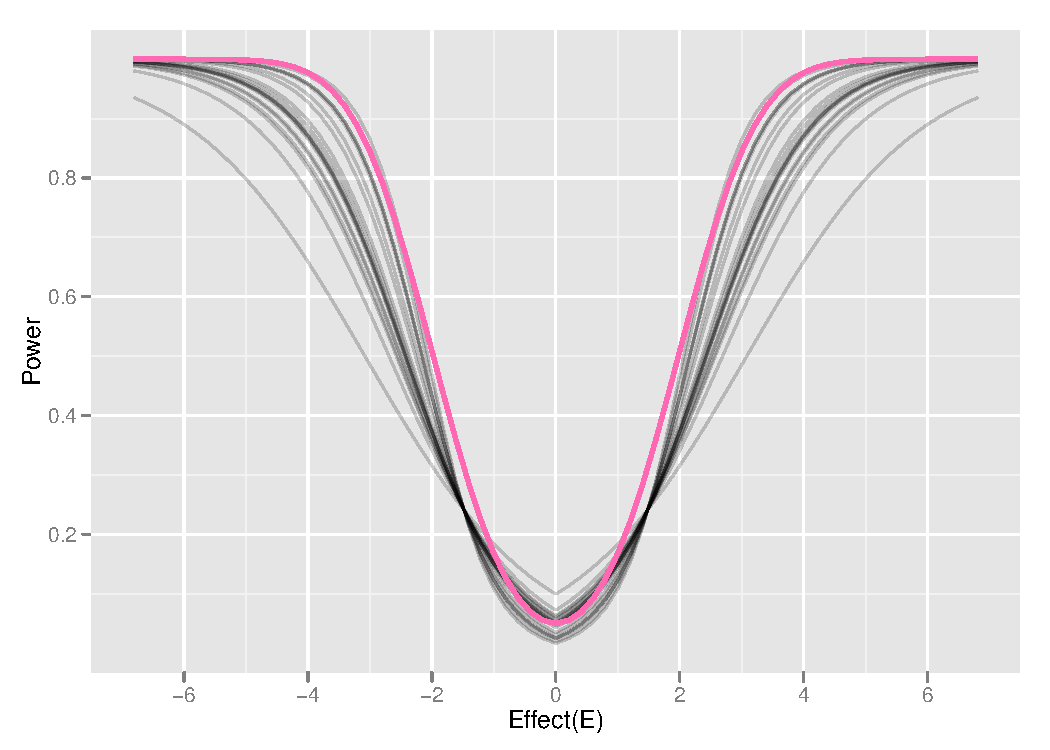
\includegraphics{effect_power_subject_exp2.pdf}}
%       \caption{Subject specific power obtained from Equation \ref{eqn:effect} and the power of UMP test for different effect size $E$ as per experiment 1 and 2.}
%       \label{fig:power_effect_subject1}
%\end{figure*}


\begin{figure*}[hbtp]
   \centering
       \scalebox{0.4}{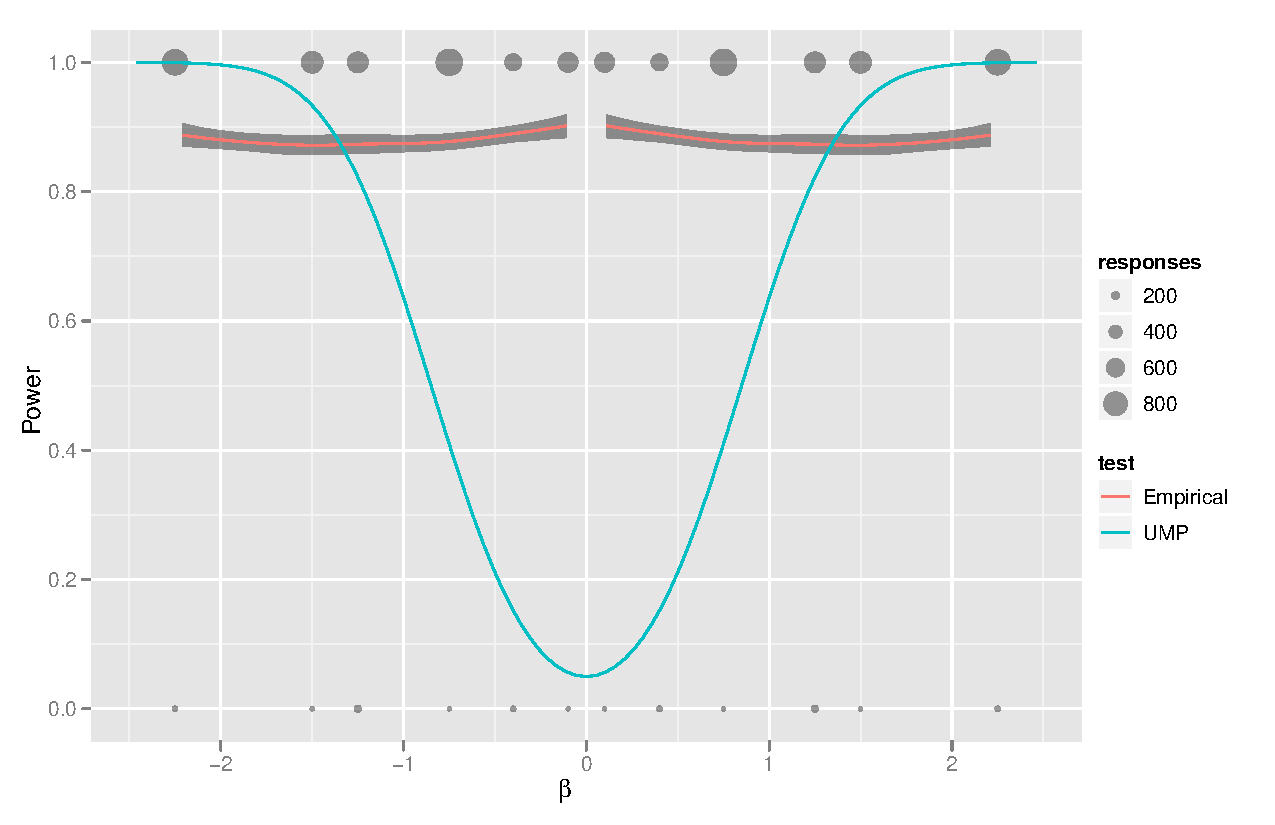
\includegraphics{power_loess_exp3.pdf}}
       \caption{Observed power shown by loess smoother with simultaneous bootstrap confidence band and the power of conventional test for sample size $n= 100$ and $\sigma = 5$ as per experiment 3. Notice that for experiment 3, power does not seem to depend on the parameter $\beta$. Di/Heike, I am not sure how I can relate this to demonstrate the power of visual inference when normal conditions are not met. Does this really test our hypothesis $H_0: \beta=0$ or some other hypothesis about the existence of cluster in the data?}
       \label{fig:power_loess3}
\end{figure*}

%\begin{figure}[hbtp]
%   \centering
%       \scalebox{0.40}{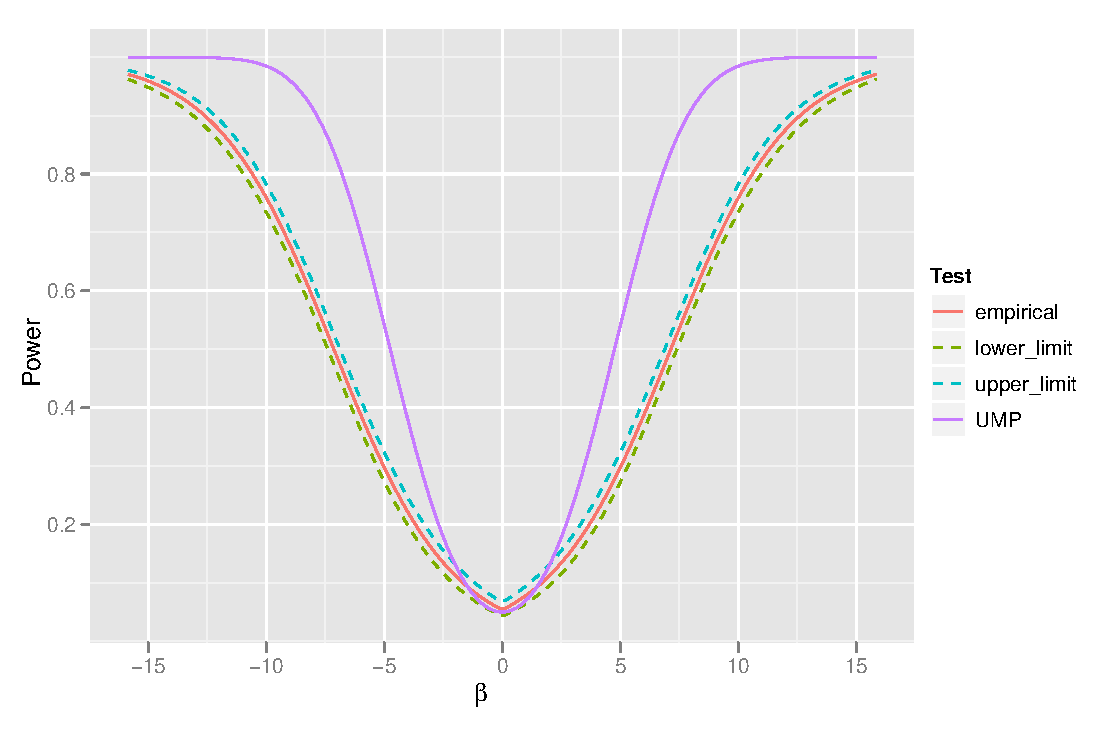
\includegraphics{power_model.pdf}}
%       \caption{Estimated power curve from Equation \ref{eqn:power} along with 95\% confidence interval for sample size $n$ = 100 and $\sigma$ = 12.  The corresponding power curve for Uniformly Most powerful (UMP) test is shown for comparison.}
%       \label{fig:power_model}
%\end{figure}

%We fit model \eqref{mixed} to the survey data obtained from the simulation experiment. The estimated overall power curve obtained from equation \eqref{eqn:power} is shown in Figure \ref{fig:power_model}. Model \ref{mixed} also gives the subject specific power curves shown in Figure \ref{fig:power_subject}. The plot includes 20 randomly selected subject-specific power curves. Notice that the power curve estimated for one subject is above the UMP test power curve. 

%\begin{figure}[hbtp]
%   \centering
%       \scalebox{0.45}{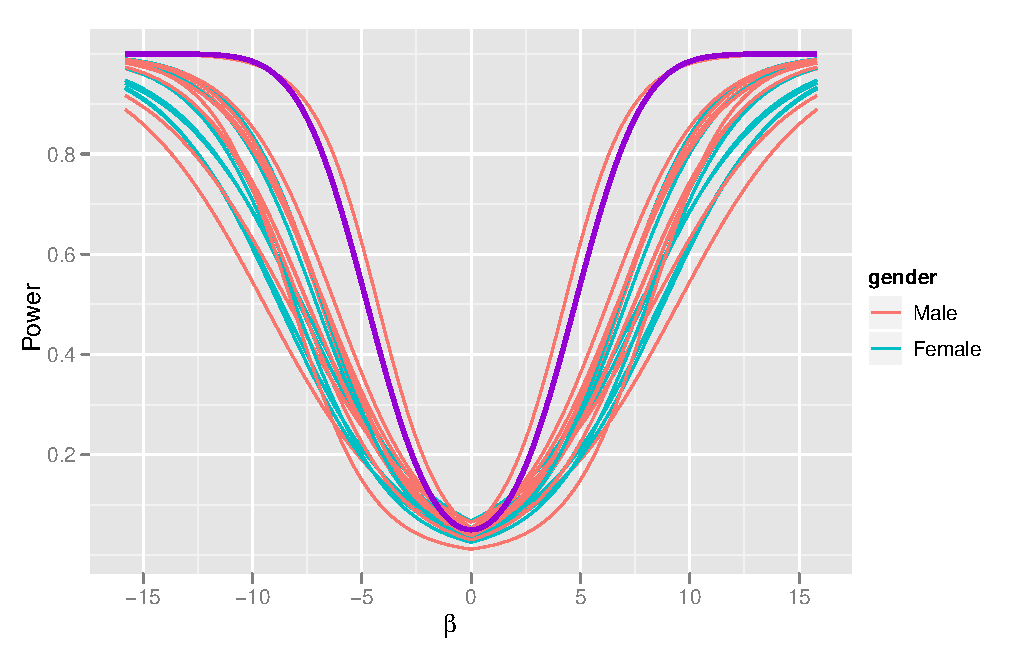
\includegraphics{power_subject.pdf}}
%       \caption{Estimated subject specific power curve from model \ref{mixed} for sample size $n$ = 100 and $\sigma$ = 12.  The corresponding power curve for Uniformly Most powerful (UMP) test is shown for comparison.}
%       \label{fig:power_subject}
%\end{figure}


\hh{From figure \ref{fig:power_loess3} we see that identification of the data plot is high independently of the effect size. This might be an indication that participants were not considering slope as distinguishing feature for the data, but the apparent clustering, i.e. the null hypothesis is being rejected, but not for the reason of the slope -- which the experimental setup was asking for --  leading to a type III error of correctly rejecting the null hypothesis for the wrong reason', as defined by \citet{mosteller:48}.} \green{Not sure that this goes here, but something needs to be said about Type III.}

\subsection{Subject-specific variation}

\begin{figure}[hbtp]
   \centering
       \scalebox{0.60}{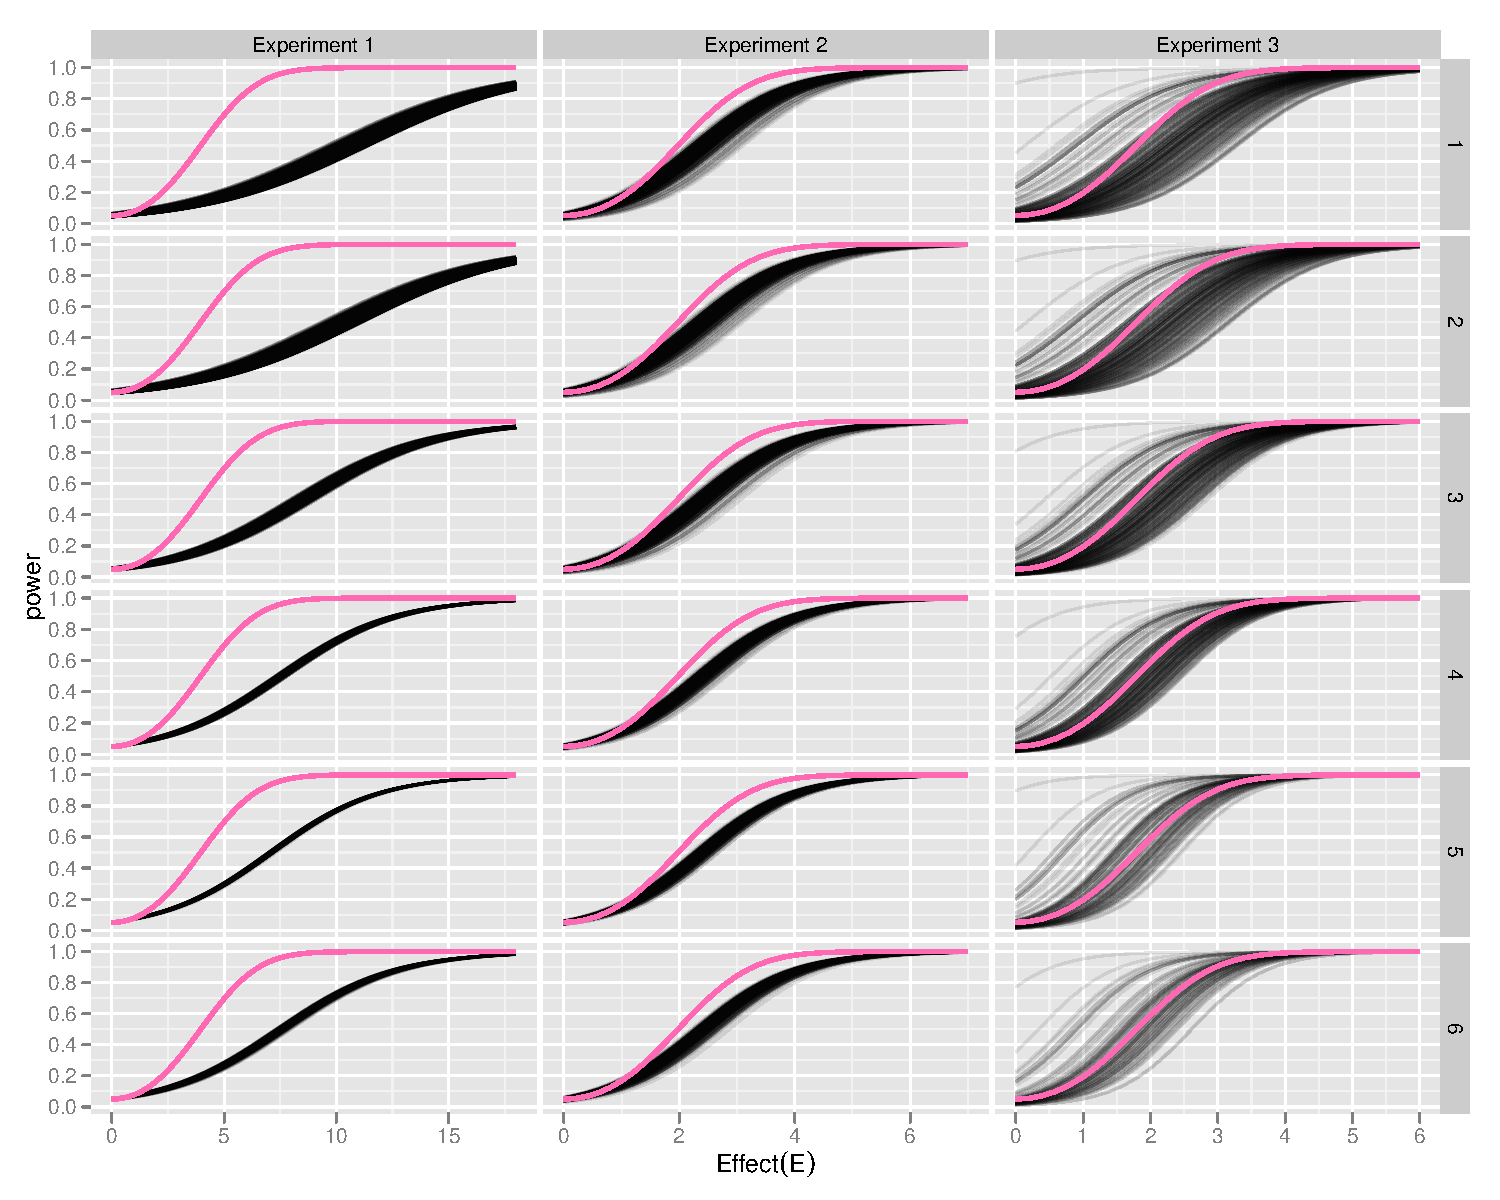
\includegraphics{power_screening_subject.pdf}}
      \caption{The subject specific power estimated from model \ref{mixed} are shown for various data sets obtained by applying 6 screening criteria.  The corresponding power curve for conventional test is shown in pink lines for comparison.}
       \label{fig:power_screening_subject}	
\end{figure}


\subsection{Estimating $p$-value in Non-Classical Settings} 

\green{third experiment doesn't really have a p-value, does it? Need to explain this. Why are there still so many small p-values in experiment 3?} \blue{$p$-values are computed fitting the full model to the contaminated data anyway.}

In the real setting, where visual inference is to be useful, there will be no classical tests or traditional $p$-values. Yet, assessing the strength of the structure is a critical component of inference. For experiments 1 and 2, to assess the signal strength we examine the proportion of correct picks, with multiple users and the $p$-value of the actual data plot. For experiment 3 the \green{How is p-value calculated here?} Figure \ref{fig:pval_pcorrect} displays scatterplots of these two variables for each experiment. As the $p$-value increases the proportion of correct responses falls, evidence of direct association between proportion of correct responses and classical test $p$-values. When $p$-value is larger than 0.15, it is almost impossible to correctly identify the observed plot in the lineup. We observed this for both experiment 1 and 2. For experiment 3, the scenario is different, because there are two structures, the association between variables, and the cluster of contaminated points.% as in this case people might have observed something other than the effect $E$.

\green{Should we use proportion of correct, rather than percentage? Wouldn't that work into the equations better?}

Yet, it is possible to obtain an estimate the strength of the signal in the actual data plot, when there are multiple evaluations, using Lemma \ref{lemma}. From Equation \ref{fig:pval_plot_signal}  we can write $1 - E[N_m]/K \approx (m-1)E[p_D] $. This gives the signal strength estimate as  
\[
\hat p_D= (1- {u}/{K})/({m-1})
\]
where $K$ is the total number of independent evaluations on a lineup and $u$ is the number of successful evaluations. Figure \ref{fig:pval_plot_signal} shows the plot signal strengths in relation with classical test $p$-values. Notice that plot signal strength is equivalent to classical test $p$-value when $p$-value is less than or equal to 0.05 and beyond that the plot signal strength levels off on a point bigger than 0.05. Thus if plot signal strength is less than 0.05, we may decide to reject the null hypothesis.



\begin{figure*}[hbtp]
   \centering
       \scalebox{0.6}{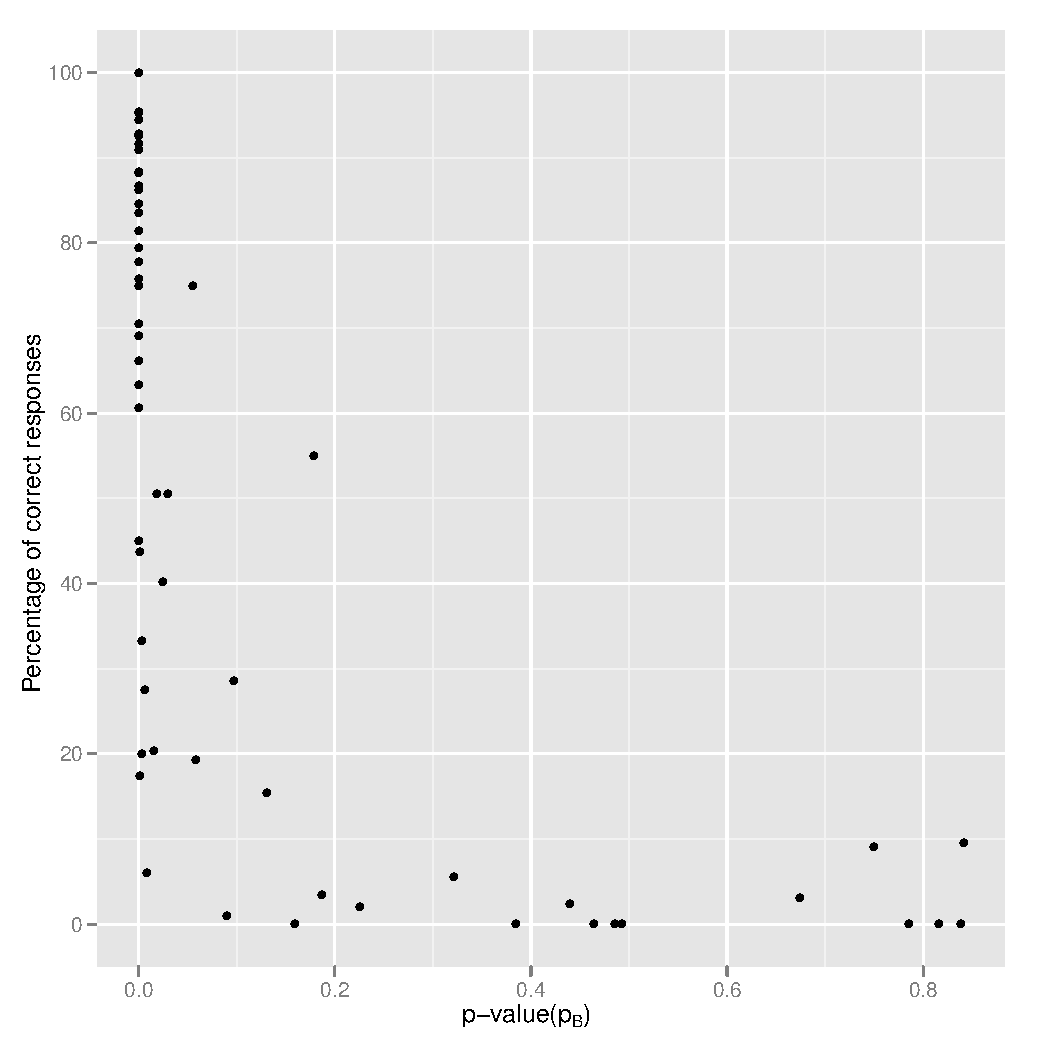
\includegraphics{p_val_percent_correct.pdf}}
       \caption{Percentage of correct responses decreases rapidly with the increase of p-value. After p-value exceeds 0.15 it is very unlikely to identify the actual plot. The theoretical justification of this is shown in figure \ref{fig:pval_power}. \blue{The scenario is different for experiment 3. $p$-value does not seem to have any effect on percent correct. This may be due to Type-III error.} \green{p-value on log scale?} }
       \label{fig:pval_pcorrect}
\end{figure*}

\begin{figure*}[hbtp]
   \centering
       \scalebox{0.6}{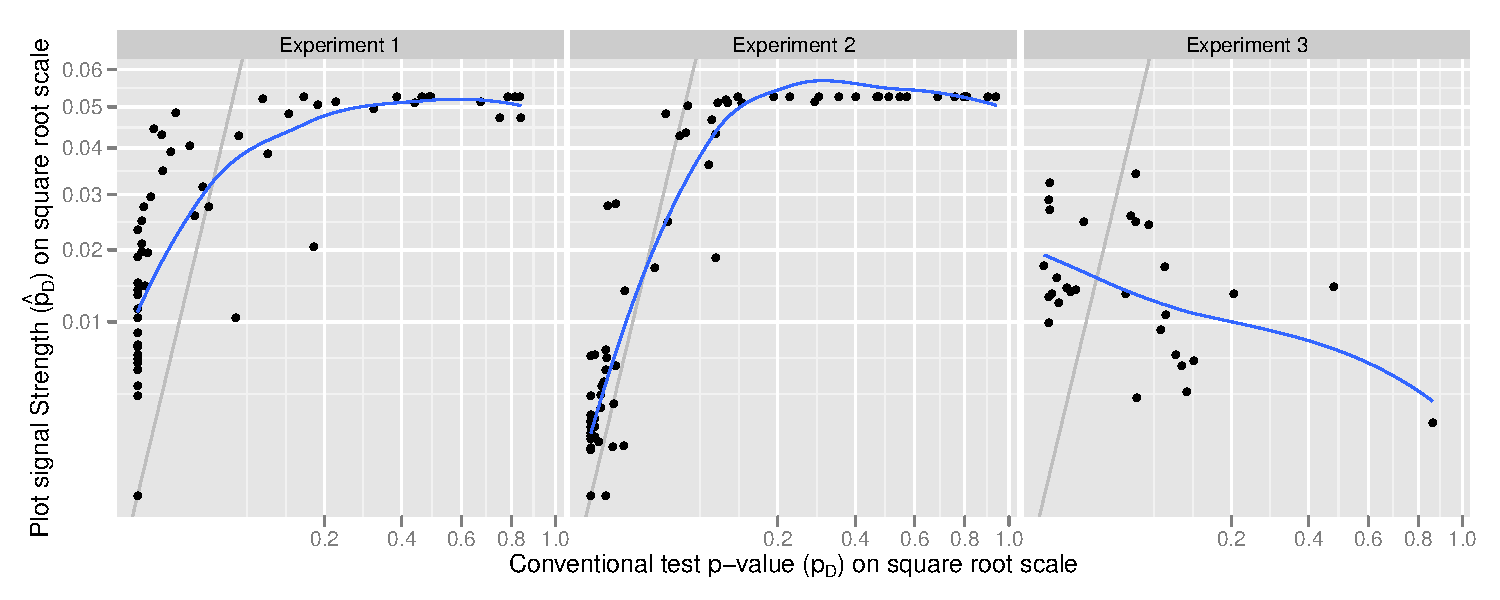
\includegraphics{p_val_plot_signal.pdf}}
       \caption{Classical test $p$-value ($p_D$) vs plot signal strength ($\hat p_D$) estimated using Lemma \ref{lemma}. The solid line is a 45 degree line which represents the equity shown in equation \ref{eqn:power_estimate}. \green{p-value on log scale?}}
       %\hh{Mahbub, could you exchange this plot for one with  $p_D$ estimated as $(1 - \#  correct/ \# shown)/(m-1)$ as given in lemma 3.1 now?}}
       \label{fig:pval_plot_signal}
\end{figure*}

\subsection{Do people tend to pick the lowest $p$-value?}

In Section \ref{sec:size} in order to make comparisons with classical tests an assumption was made that the observer would pick the plot in the lineup that had the lowest $p$-value. In this section we take a look at the picks that subjects made, to see if this is, indeed, true. Figure \ref{fig:P-val_rank} shows side-by-side boxplots of rank of plot (in its lineup) and how many subjects selected the plot. \green{Maybe we don't need this plot.} 

Figures \ref{fig:P-val_log} and \ref{fig:P-val_log2} show the selection counts and $p$-values of all plots for each lineup in experiments 1 and 2, respectively. In each of these plots, the log of $p$-value for each plot in the lineup is plotted horizntally and the count of the number of subjects who selected this plot is displayed vertically. The dot represents this point, and the lines connect vertically with 0 count. Each row corresponds to a different $\beta$ value ordered top to bottom from lowest to highest. Columns correspond to the other levels of the exeriment, sample size $(n)$, error standard deviation $(\sigma)$ and replicate. (Empty cells indicate no lineup shown with this combination.) Red indicates the actual data plot, which is not always the plot in the lineup with the lowest $p$-value. In both experiments as $\beta$ gets larger (stronger effect) people tended to select the plot with the lowest $p$-value. This is less so the case when $\beta$ is small, when standard deviation is large and sample size is small. The results are clearer for experiment 2, that used a continuous covariate. So for most observers, the assumption that they pick the plot with the smallest $p$-value would appear to be reasonable, and the actual power of the visual test should be close to the expected power.

Experiment 3 does not have $p$-values associated with each plot, so the assumption can only be tested with the first two experiments. Practically, this is not an assumption that is explicitly made, because there will not be a $p$-value available. Rather it is assumed that the observer has the ability to select the plot with the most extreme structure. A few of the lineups indicated that occasionally people cue on different patterns, for example, in experiment 1 the lineup $\beta=0, n=100, sd=5, rep=1$ (first row, fourth column) many subjects chose the same plot, that had a higher $p$-value. Some of these anomalous lineups were selcted for follow-up studies using an eyetracker to investigate what people were looking at.

%Number of lineups for which most of the subjects picked the data plot based on the minimum $p$-values are shown in table \ref{tbl:pval_assumption} for both experiment 1 and 2. The $p$-values of lineups which were not chosen based on minimum $p$-value are also very small (close to minimum) as we see in both figures \ref{fig:P-val_log} and \ref{fig:P-val_log2}. We see the same pattern in figure \ref{fig:P-val_rank} where the median number of people who pick the data plot with minimum $p$-value (rank 1) are much higher than other ranks.

%\begin{table}[hbtp]
%\caption{Number of lineups for which most people pick the plot with minimum $p$-value. The data used is from screening criteria 1. } 
%\begin{center}
%\begin{tabular}{cccc}
%  \hline
%screening & Experiment & Total &  minimum $p$-value\\ 
%criteria & & lineups & picked by the most \\
%  \hline
%   & 1 &  60 &  37 \\ [-1ex]
%    \raisebox{1.5ex}{1} & 2 &  70 &  60 \\ 
%\hline
%     & 1 &  60 &  38 \\  [-1ex]
%    \raisebox{1.5ex}{2} & 2 &  70 &  61 \\ 
%\hline
%     & 1 &  60 &  38 \\  [-1ex]
%   \raisebox{1.5ex} {3} & 2 &  70 &  60 \\ 
%\hline
%     & 1 &  60 &  41 \\  [-1ex]
%    \raisebox{1.5ex}{4} & 2 &  70 &  60 \\ 
%\hline
%     & 1 &  60 &  39 \\  [-1ex]
%    \raisebox{1.5ex}{5} & 2 &  70 &  60 \\ 
%\hline
%     & 1 &  60 &  40 \\  [-1ex]
%    \raisebox{1.5ex}{6} & 2 &  70 &  60 \\ 
%   \hline
%\end{tabular}
%\end{center}
%\end{table}



\begin{table}[hbtp]
\caption{Number of lineups for which most people pick the plot with minimum $p$-value.  } 
\begin{center}
\begin{tabular}{ccc} \hline
screening & \multicolumn{2}{c} {lineups picked by minimum $p$-value} \\
 \cline{2-3}
criteria & Experiment 1 & Experiment 2 \\ 
  \hline
1 & 37 & 60 \\ 
2 & 38 & 61 \\  
3 & 38 & 60 \\ 
4 & 41 & 60 \\ 
5 & 39 & 60 \\
6 & 40 & 60 \\ 
\hline
Total lineups & 60 & 70 \\  
\hline
\end{tabular}
\end{center}
\label{tbl:pval_assumption} 
\end{table}

\begin{figure*}[hbtp]
   \centering
       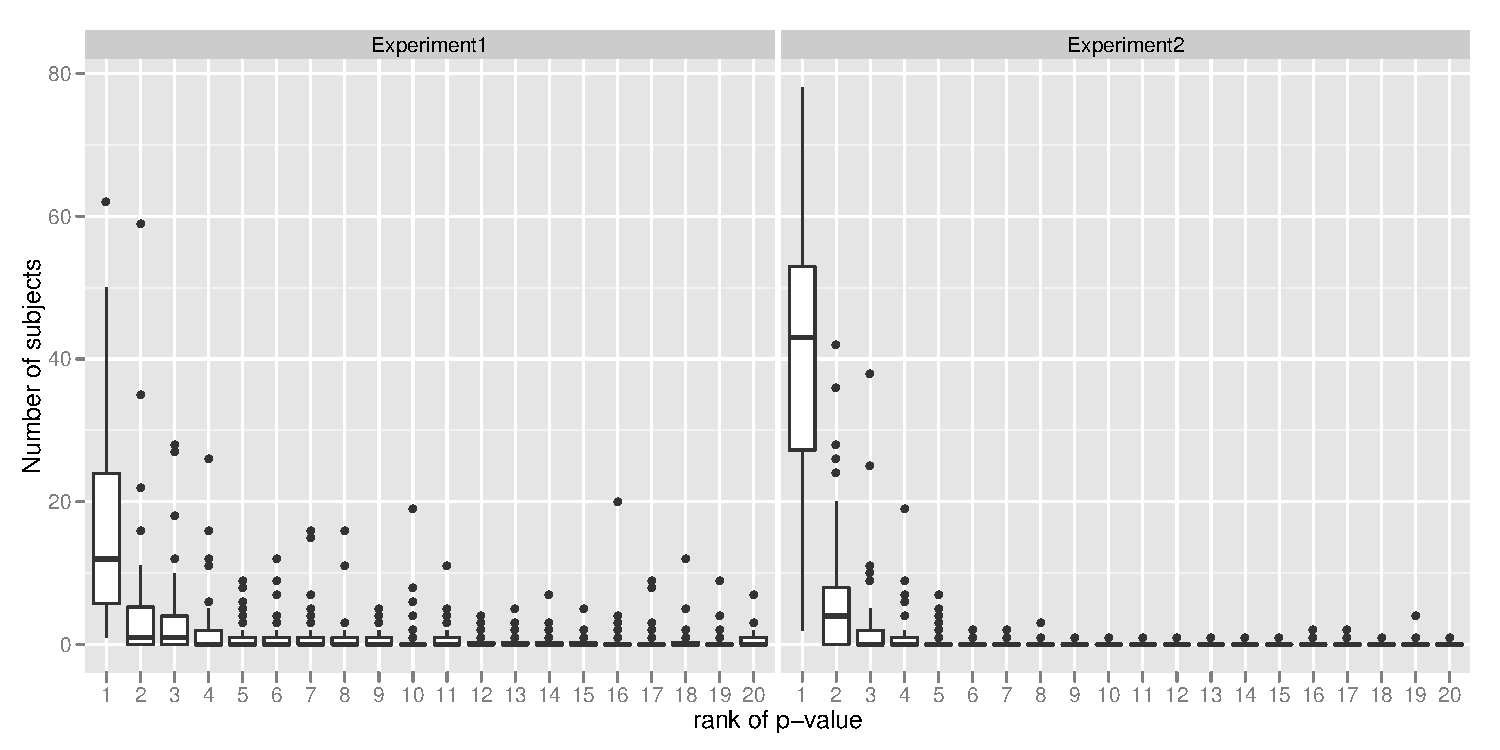
\includegraphics[width=0.95\textwidth]{p_val_rank_counts12.pdf}
       \caption{Rank of p-values in a lineup of size 20 and the number of subjects choosing that plot in the lineup of experiment 1 and 2 with raw data (screening criteria 1). This indicates that most of the subjects pick the plot with minimum p-value (rank 1). There are subjects choosing the lineups with highest p-value(rank 20) but we can attribute this behavior to the type-I error. Can we?  \green{Maybe don't need this plot}}
       \label{fig:P-val_rank}
\end{figure*}

\begin{figure*}[hbtp]
   \centering
       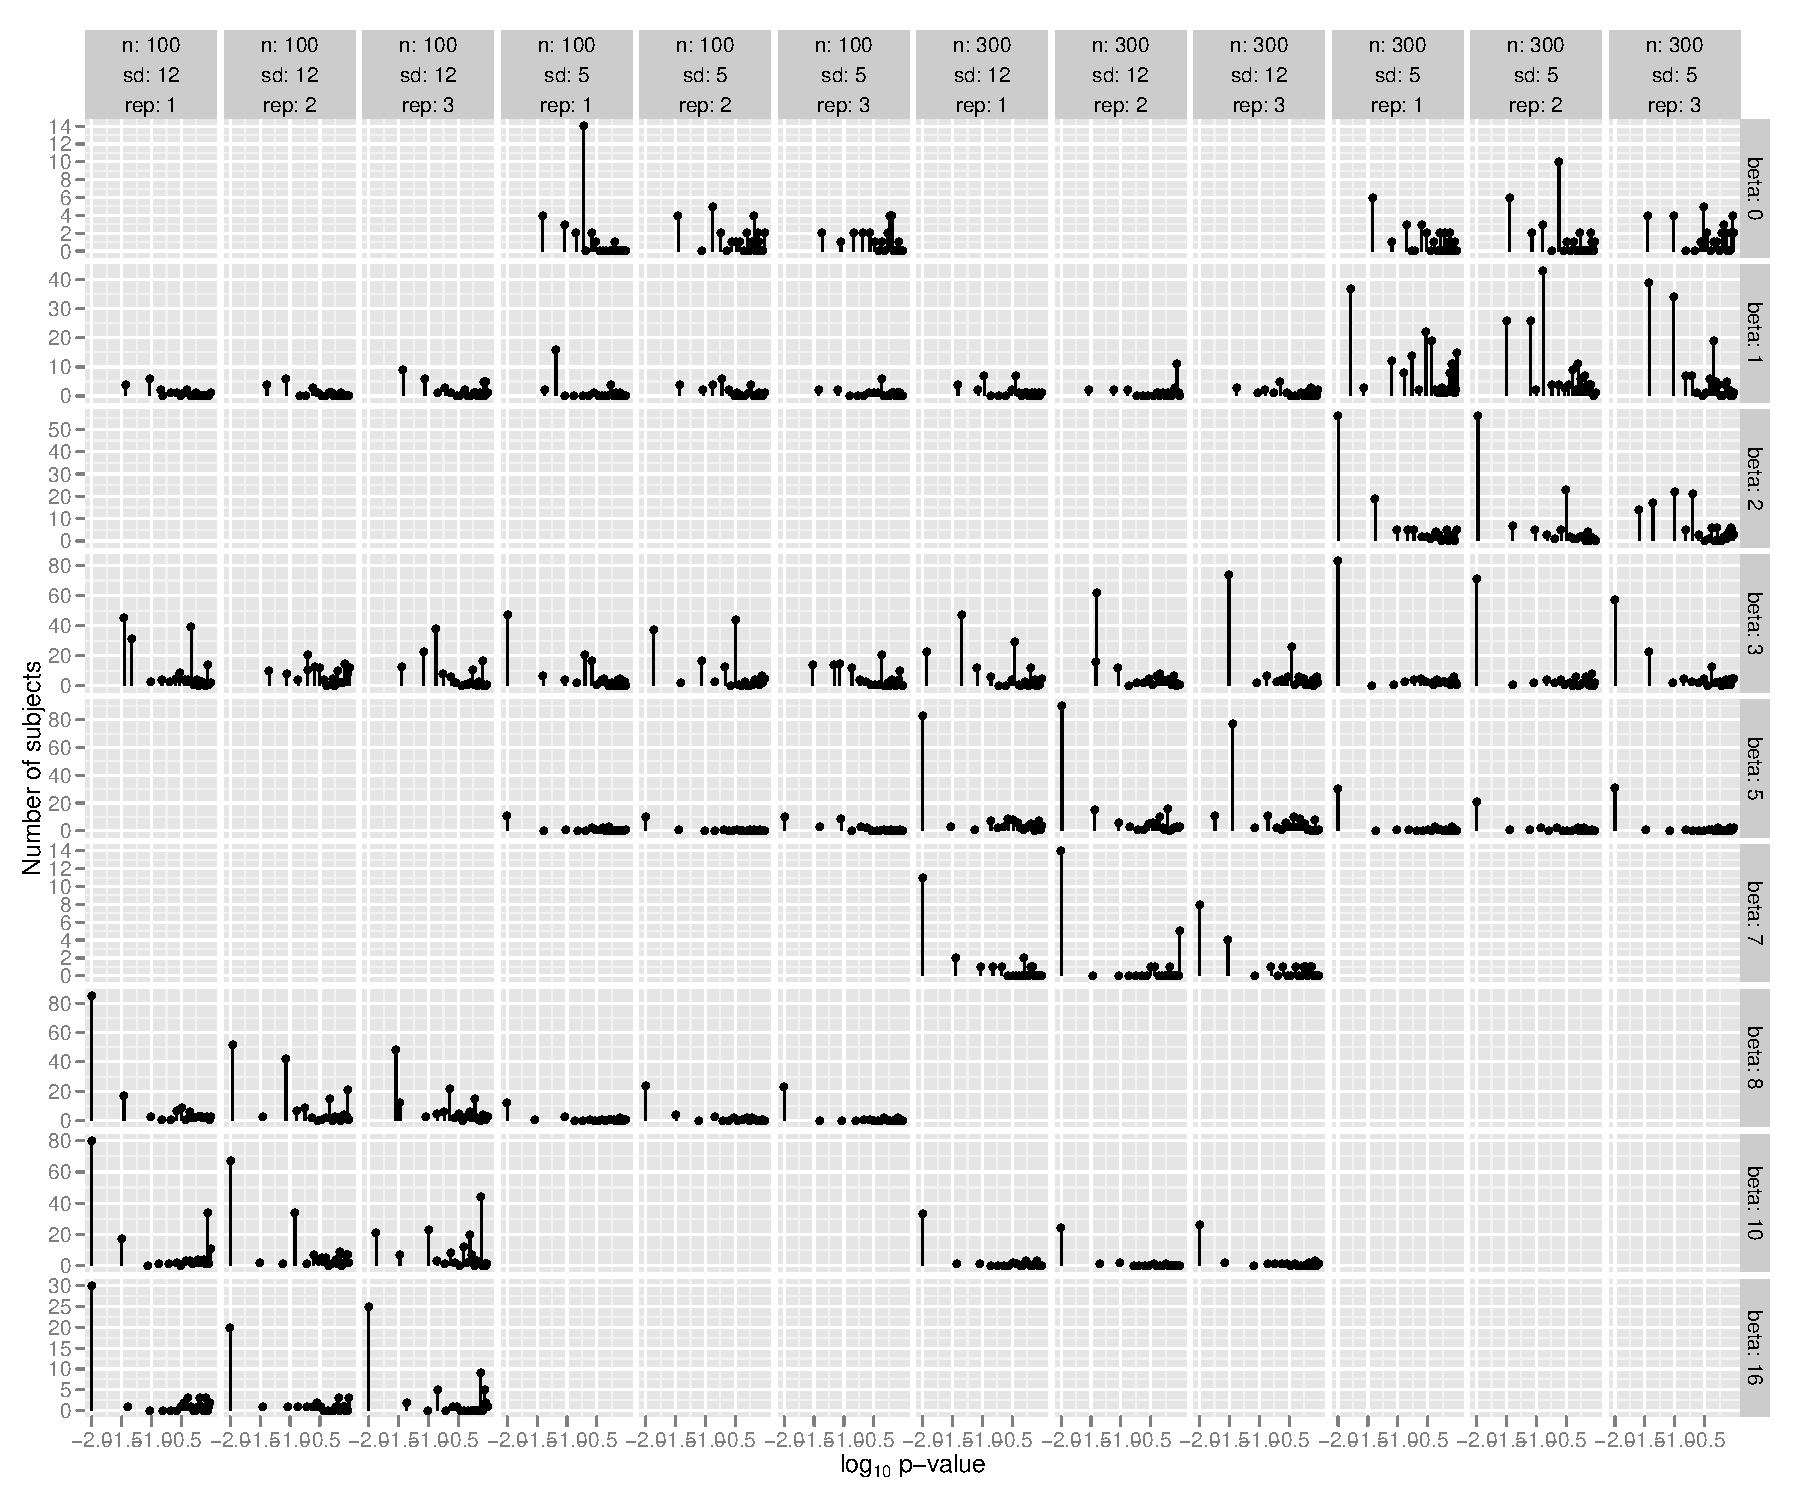
\includegraphics[width=0.95\textwidth]{p_val_log_counts.pdf}
       \caption{Relative frequency of plot picks compared to other plots in the lineup plotted against the $p$-value (on log$_{10}$ scale) of each plot for all of the sixty (60) individual lineups for experiment 1. The colored lines indicate the plot with the lowest $p$-value. Rows correspond to $\beta$, smallest to largest values from top to bottom. Columns correspond to other experimental treatments, sample size $(n)$, error standard deviation $(\sigma)$, and replicate. Empty cells indicate no lineup for that combination of parameters. Highest counts tend to be the plot in the lineup having the lowest $p$-value.}
       \label{fig:P-val_log}
\end{figure*}

\begin{figure*}[hbtp]
   \centering
       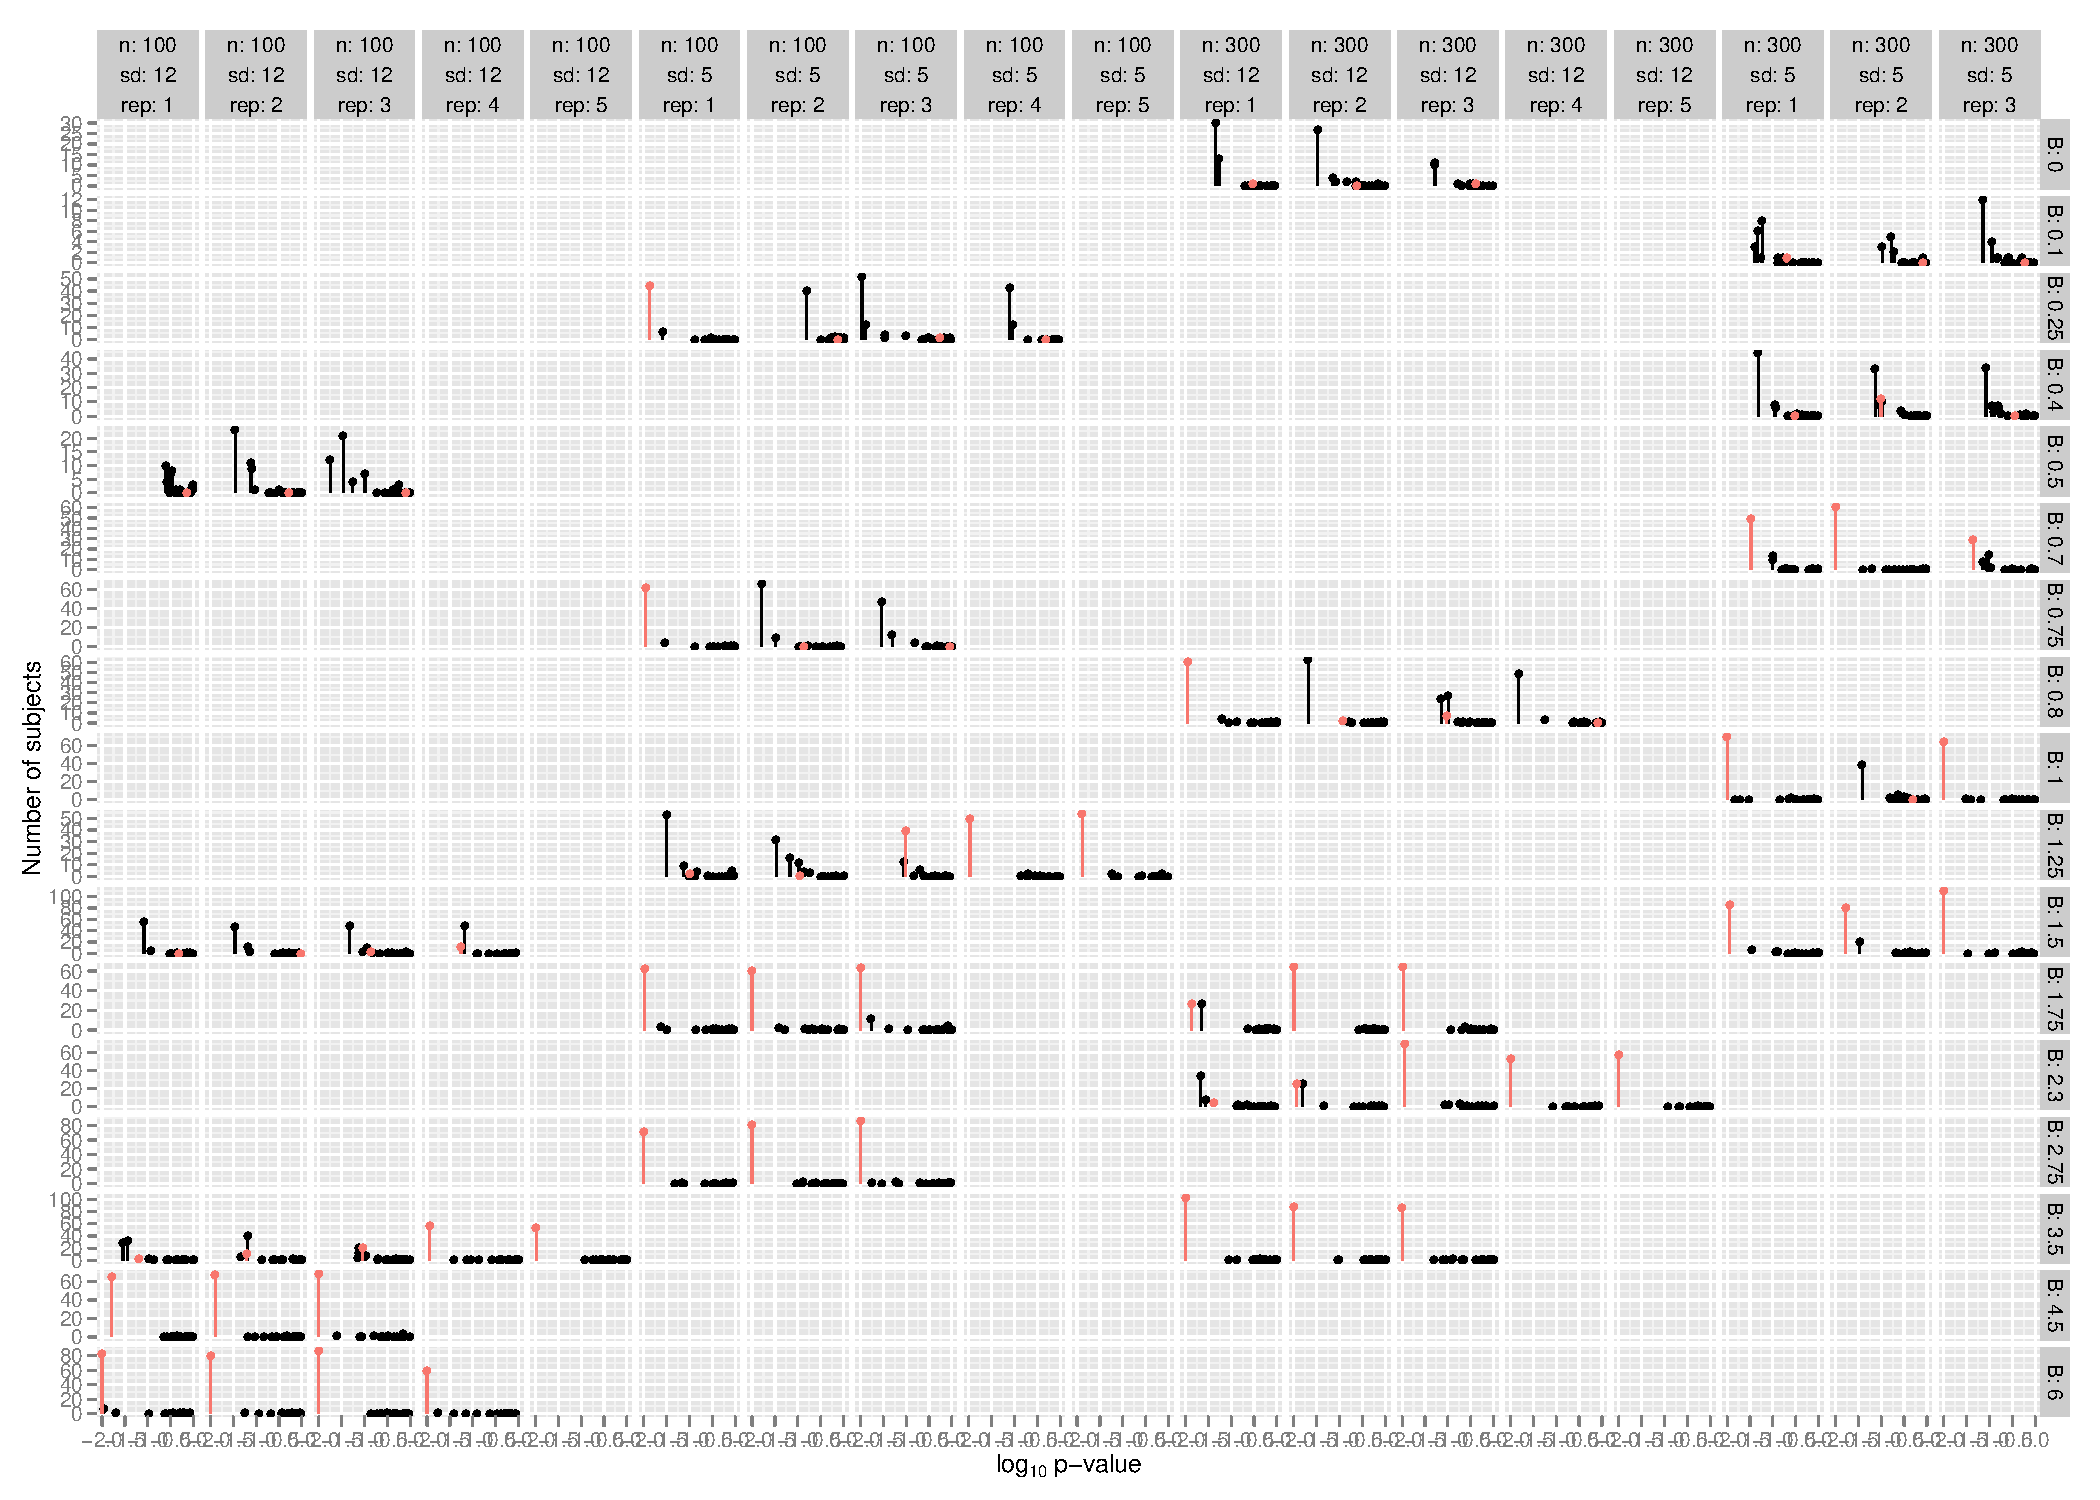
\includegraphics[width=0.95\textwidth]{p_val_log_counts2.pdf}
       \caption{Relative frequency of plot picks compared to other plots in the lineup plotted against the $p$-value (on log$_{10}$ scale) of each plot for all of the seventy (70) individual lineups for experiment 2. The colored lines indicate the plot with the lowest $p$-value. Rows correspond to $\beta$, smallest to largest values from top to bottom. Columns correspond to other experimental treatments, sample size $(n)$, error standard deviation $(\sigma)$, and replicate. Empty cells indicate no lineup for that combination of parameters. Highest counts tend to be the plot in the lineup having the lowest $p$-value, even more so than for experiment 1.}
       \label{fig:P-val_log2}
\end{figure*}


\section{Conclusions}

The purpose of this paper has been to examine the effectiveness of visual inference methods in direct comparison to existing inference methods. We need to be clear that this is not the purpose of visual inference generally: visual methods should not be seen as competitors to traditional inference.  The purpose here, is to  establish properties and  efficacy of visual testing procedures in order to use them in situations where traditional tests cannot be used. For this experiment the effect of $\beta_2$ was examined using side-by-side boxplots. Future experiments will be conducted to compare other regression parameters as described in Table \ref{tbl:stat_multiple} and assess sensitivity of power to modeling conditions.

\paragraph{Acknowledgement:}

This work was funded by National Science Foundation grant DMS 1007697.

%\bibliographystyle{plain}
%\bibliographystyle{plainnat}
\bibliographystyle{asa}
%\bibliographystyle{ieeetr}
\bibliography{references}

%\end{multicols}
\section*{Appendix}

\begin{table}[hbtp]
\caption{Selection of 10 lineups for a person to evaluate in the simulation experiment with discrete covariate described in section \ref{sec:category}.} 
\centering
\begin{tabular}{c c c c  c c c}
\hline\hline
Difficulty& \multicolumn{3}{c}{parameter combination}& Number of evaluations &Total number  & number of lineups\\
level & $n$ & $\sigma$ & $\beta$ &required($n_{\gamma}$) & of lineups & randomly shown \\
\hline
easy&100& 5&8 & 1& 12 & 1\\
&100&12&16 &1&&\\
&300& 5&5 &1&&\\
&300&12&10 &1 &&\\
\hline
medium&100& 5&3 &203 & 9 &2\\
&300& 5&2,3 & 97, 1&&\\
\hline
hard&100&12&3,8,10 & 277, 126, 23& 18 &6\\
&300& 5&1 & 371 &&\\
&300&12&3,5& 375,74 &&\\
\hline
mixed&100& 5&1,5,0& 214, 2,73 & 21 &1\\
&100&12&1& 100& &\\
&300& 5&0 & 73&&\\
&300&12&7,1& 2, 152&&\\
\hline
Total &&&&&60&10\\
\hline
\end{tabular}
\label{tbl:dist_lineup1}
\end{table} 

\end{document}  %End of document.





\begin {abstract} 
Statistical graphics play a crucial role in exploratory data analysis, model checking and diagnosis. Until recently there were no formal visual methods in place for determining statistical significance of findings. This changed, when Buja et al.(2009) conceptually introduced two protocols for formal tests of visual findings. In this paper we take this a step further by comparing the lineup protocol (Buja et al.2009) against classical statistical testing  of the significance of regression model parameters. A human subjects experiment is conducted using simulated data to provide controlled conditions. Results suggest that the lineup protocol provides results equivalent to the conventional test and for some scenarios yields better power than the conventional test.
\end {abstract}

\end{document}
